\documentclass[a4paper,10pt]{article}

%\usepackage[utf8]{inputenc} 
%\usepackage[square,sort,comma,numbers]{natbib}
%\usepackage[backend=biber,autocite=inline,style=authoryear]{biblatex}
\usepackage[backend=biber,autocite=inline]{biblatex}
\addbibresource{mybib.bib}
\usepackage{a4wide}
\usepackage{amsmath}
\usepackage{amssymb}
\usepackage{amsthm}
\usepackage{listings}
\usepackage{color}
\usepackage{enumerate}
%\usepackage{IEEEtrantools}
%\usepackage[redeflists]{IEEEtrantools}
\usepackage{verbatim}
\usepackage{graphicx}
\usepackage{subcaption}
\usepackage[section]{placeins} %no trans-sectional figures!
\usepackage{wrapfig, framed, caption}

\usepackage{booktabs} % For \toprule, \midrule and \bottomrule
\usepackage{siunitx} % Formats the units and values
\usepackage{pgfplotstable} % Generates table from .csv
% Setup siunitx:
\sisetup{
  round-mode          = places, % Rounds numbers
  round-precision     = 2, % to 2 places
}

\usepackage{hyperref}
\hypersetup{linktocpage,
            linktoc=all,
            colorlinks=true,
            linkcolor=blue,
            }

\usepackage{lipsum}
%\usepackage[onehalfspace]{setspace}
\usepackage{setspace}

% Basic data
\newcommand{\N}{\mathbb{N}}
\newcommand{\C}{\mathbb{C}}
\newcommand{\ASSIGNMENT}{2}
\newcommand{\B}{\{-1,1\}}
\newcommand{\E}{\mathbf{E}}
\newcommand{\F}{\mathbb{F}}
\newcommand{\Inf}{\textbf{Inf}}
\newcommand{\I}{\mathbf{I}}
\newcommand{\NS}{\textbf{NS}}
\newcommand{\R}{\mathbb{R}}
\newcommand{\Z}{\mathbb{Z}}
\newcommand{\aufgabe}[1]{\item{\bf #1}}
\newcommand{\bvec}[1]{\mathbf{#1}}
\newcommand{\bv}[1]{\mathbf{#1}}
\newcommand{\ceil}[1]{\lceil{#1}\rceil}
\newcommand{\floor}[1]{\lfloor{#1}\rfloor}
\newcommand{\gt}{>}
\newcommand{\half}[1]{\frac{#1}{2}}
\newcommand{\lt}{<}
\newcommand{\tuple}[1]{\langle #1 \rangle}

\newcommand{\suftab}{\text{suftab}}

\setlength{\parskip}{1.0em}
\setlength{\parindent}{1em}


\lstset{
%basicstyle=\footnotesize,
%basicstyle=\ttfamily\footnotesize,
%basicstyle=\ttfamily\small,
%basicstyle=\ttfamily\scriptsize,
frame=single,
%numbers=none,
%numbersep=5pt,
numberstyle=\tiny,
showspaces=false,
showstringspaces=false,
tabsize=2,
breaklines=true,
%escapeinside={#*}{*#},
escapeinside={$}{$},
%escapeinside={*\&}{\&*},% if you want to add LaTeX within your code
%mathescape=true,
%language=C++
}

\theoremstyle{definition}
\newtheorem{mydef}{Definition}[section]

\theoremstyle{remark}
\newtheorem{remark}{Remark}

\theoremstyle{plain}
\newtheorem{thm}{Theorem}[section]
%\newtheorem{thm}{Theorem}[mydef]
\newtheorem{lemma}{Lemma}[section]
%\newtheorem{lemma}{Lemma}[mydef]

\begin{document}
\renewcommand{\thesubsection}{\thesection.\alph{subsection}}\renewcommand{\thesubsection}{\thesection.\alph{subsection}}


% Document title
\newpage% Document title
\begin{titlepage}
	\centering
%    \title{Bachelorthesis about Network Propagation}
%    \author{Yiftach Kolb}
%    \date{\today}
%    {\bf\LARGE Freie Universität Berlin and MPIMG}
    {\bf\large Freie Universität Berlin and
    Max Planck Institute's MPIMG}
    \par Department of Bioinformatics
    {\scshape\LARGE \par Partially Labeled
    Classification in Graphs}
    {\scshape\Large\par Using Network Propagation Methods 
    \par and Applications in Protein Function Annotaions}
    \vfill
  	{\Large Yiftach Kolb \par}
    {yiftach.kolb@fu-berlin.de}
    \vfill
  	{\Large a Bachelor Thesis\par}
    \vfill
	  {\Large Supervisor: \par
    Prof. Dr. Martin Vingron, \normalsize vingron@molgen.mpg.de 
    \par}
    {\large \today\par}
\end{titlepage}



%abstract
\begin{abstract}
This is an abstract \dots
\end{abstract}

%toc
\tableofcontents

%Introduction
\newpage %Introduction
\section{Introduction}

In this paper we propose a protein function prediction algorithm,
which in essence works similarly to the adage ''Tell me who your
friend are, and I will tell you who you are''. Imagine that we can
accurately predict the function of a protein in the cells of an
organism bases on its biochemical interactions with the other
proteins, and the interactions of the other proteins between
themselves. This has in fact demonstrated to be true by
\textcite{schwikowski2000network}. But we are trying to improve on
it. In the formulation of the adage above, We want to tell you who
you are based on information on some friends of your friends. 
We want that because in the world of protein research, there are
still many that are unresearched or mostly unresearched.

The specific problem we are dealing here, from the perspective of
bioinformaticians, is of protein function prediction in a
protein-protein interaction network (PPIN), yet the actual algorithm
is more general and applies to any network really. For this reason
why we call the problem 'Partially labeled classification' (PLC) as it was
named by \textcite{szummer2002partially}.

Our proposed algorithm uses the network propagation method of random
walk with restart (RWR). These methods has been used most famously
by Google for their search algorithm but also in bioinformatics  for
example for 'disease module identification' by
\cite{vandin2012discovery, barel2020netcore}.

We wanted to make this paper somewhat self contained and therefore
we included the mathematical background of stochastic matrices and random walk
with restart in the first 2 sections as well as in the 3 appendices.
The are intended to provide a 'feel' for the RWR process,
as well as to 
intercept some possible questions, likely even by the author
within a few decades from now, about random walks and stochastic matrices.
%We dedicate sections 2 and 3 of this Thesis to explain the
%underlying mathematical theories of stochastic matrices and random
%walk with restart in graphs. 
These sections are largely going according to textbooks
from \textcite{meyer2000matrix} and \textcite{herstein_winter_1989}.
%The purpose is to make this work somewhat self standing with the
%mathematical foundations it is based on, to give a 'feel' for how
%RWR actually work, 
We included some 
lemmas that prove why we can use RWR it in the networks we are dealing
with. These two sections are expanded by appendices 1 and 2.

Section 4 deals with the subjects
of community structure and spectral clustering in graphs. There is
a great deal of overlap between the PLC problem and community structure. 
Essentially the function prediction algorithm is based on the
paradigm that proteins of the same functional classification do tend
to form 'communities' within the PPI. We therefore first propose and
test a heuristic for graph clustering, because if it doesn't work
there is no reason that our approach has any hope resolving the PLC.
We also provide in appendix 3 some details about spectral clustering
and compare it with the heuristic.

In section 5 we propose an algorithm for protein function prediction
(or more generally for the partially labeled classification
problem). We try and compare several clustering methods and then
carry forward more test with the method of choice.

Finally in section 7 we draw some conclusions, discuss other
methods and approaches, and consider possible ways to carry with
this research forward.


%section
\newpage \section{Linear algebra primer}

\subsection*{Prologue}
This section is mostly based on \cite{meyer2000matrix} and
\cite{herstein_winter_1989}. We are going to have to use allot of
definitions anyway and cite big theorems like the Perron-Froebenius
theorems, so we might as well provide an
understanding of the important properties of stochastic matrices
which we need for the RWR methods.

This chapter is accompanied by an appendix chapter, which containes
more material and presents proofs or sketch of a proof to most
theorems and lemmas.
We try to keep the chapter intself short and just mention theorems
and properties that are strictly necessary for the following
chapters.

This chapter together with the appendix
is also meant to intercept likely questions, quite possibly even by
by the author himself within a few decades from now, such as, 'what if we
consider complex vectors, maybe there is a complex eigenvalue who is
greater than 1 ?', no there isn't, read here why.

\subsection*{Theory}

\begin{mydef}
\label{def:transition} A \textbf{Transition Matrix } (we call
it a \textbf{Transition} in short), which is sometimes also called a
\textbf{stochastic matrix}, is a real valued non negative square
($n \times n$) matrix $A$ such that each of its columns sums up to one: $$A
\geq 0,\ \forall j \sum_i A_{i,j} = 1$$ $A$ acts from the left as a
linear mapping: $A:v \to A \cdot v$. In this paper we use left
multiplication convention ($Av$). There are many other publications
that deal with random walk and Markov processes, where right
multiplication is used ($v \cdot A$), and accordingly the rows are
normalized rather than the columns.

A transition is \textbf{positive}, designated by $A > 0$ if all its entries are positive.

A transition is \textbf{primitive} if for some $k>$ $A^k$ is positive. The same
property is called \textbf{regular} in some other sources.

A transition is \textbf{irreducible} if for every entry $A_{i,j}$ there is some $k$ such
that $A^k_{i,j} > 0$.

It can be shown that 
A matrix $A$ is 
irreducible by and only if it is NOT
similar by permutations matrices to a block upper triangular matrix
which means 
$
\nexists P : 
A =
P
\begin{pmatrix}
B & C \\
0 & D
\end{pmatrix}
P^{-1}
$

where $P$ is a permutation matrix and $B, C$ are square matrices of size greater than $0$.
\end{mydef}

\begin{mydef}
\label{def:state}
A \textbf{State} is a non-negative vector $v \in R^n$ s.t $\sum_i v_i = 1$.
\end{mydef}

\begin{remark}
\label{remark:state}
If $v$ is a
state and $A$ is a transition as defined in
\ref{def:transition}, then
  $Av$ is also a state because: 
$$\sum_i(Av)_i = \sum_j v_j(\sum_k A_{j,k}) = \sum_j v_j \cdot 1 = 1$$
Also its easy to confirm by multiplying with $e_i$, that if $Av$ is a state
for every state $v$ 
each column $A e_i$ must sum to $1$.
Therefore this is an equivalent definition for a transition.

If $A$ is a transition and $x,y$ are two states such that
$x \leq Ay$ then $x=y$.
\end{remark}

\begin{mydef}
\label{def:abs}
%changed C to R per Martin's request but it holds for C
Given $A \in \R^{n \times n}$ We let $|A| \in \R^{n \times n}$ be the resulting
matrix from applying $|\cdot|$ element wise. Given a vector $v \in \C^n$ we let
$|v| \in \R^n$ the corresponding non-negative vector.

We also let $A \gt 0, v \gt 0$ mean that it holds coordinate wise. 
\end{mydef}

Here is a very useful lemma for non-negative matrices which we will need later:
\begin{lemma}
\label{lem:eqal_by_vector}
Let $0 \leq A \leq B \in \R^{n \times n}$ 
and let $0 \lt v \in \R^n$.
If $Av = Bv$ then $A = B$.
\begin{proof}
Trivial.
\end{proof}
\end{lemma}

\begin{remark}
\label{remark:abs}
If $u \in \C^n$ is on the unit circle and $T$ a transition then
$|u|$ is a state, meaning $\||u|\|_1=1$, so $T|u|$ is also a state 
so $\|T|u|\|_1=1$.

We have (component-wise) $|Tu| \leq T|u|$. If $T>0$ and $u$ has negative or
non-real entries, then this inequality must be strict and
then $\|Tu\|_1 \lt \|T|u|\|_1 = 1$.
\end{remark}

\begin{lemma}
\label{lem:exist1}
If $T$ is a transition, then
there is a state $u$ such that $Tu = u$.
\begin{proof}
In the appendix
\end{proof}
\end{lemma}


\begin{lemma}
\label{lem:uniq1}
If a transition $A \gt 0$ (or primitive)
, then it has exactly
one eigenvector $v$ with eigenvalue $1$ and in addition $v$ can be
chosen to be strictly positive.
Furthermore, for any other eigenvalue
$\lambda$ it holds that $|\lambda| \lt 1$.

If $A$ is just irreducible then then again $v>0$ and is unique but there may be
additional eigenvalues on the unit circle.

\begin{proof}
In the appendix
\end{proof}
\end{lemma}

\begin{remark}
\label{remark:rhoisone}
The lemmas and theorems in this section are phrased in term of transitions. They
hold true in the more general case of positive/non-negative
linear transformations and one just replaces $1$ with the \textbf{spectral
radius} $ \rho = \rho(A)$.

In general a non-negative linear transformation has a \textbf{spectral radius}
$\rho = \rho(A)$ which is the absolute value of its greatest eigenvalue. In the case of
positive maps there is a unique single eigenvector with $\rho$ as the unique
greatest eigenvalue and so forth \dots. When we deal with a transition map,
lemma \ref{lem:uniq1} guaranties 
it has a spectral value of $\rho(A) = 1$.
\end{remark}

\begin{thm}
\label{thm:transition_ev}
Let $T$ be a positive (or primitive) transition. Then 

1. $1$ is the greatest eigenvalue
of $T$ and it has one unique eigenvector which is also positive,
so there exists a unique stationary state.

2. All the other eigenvalues have absolute value strictly less than $1$.

3. For every state $u$, $T^ku$ converges to the stationary state $\pi$.
In particular the columns of $T^k$ converge to $\pi$.

\begin{proof}
In the appendix
\end{proof}
\end{thm}

\begin{thm}
\label{thm:transition_irr_ev}
Let $T$ be an irreducible positive (or primitive) transition. 
Then:

1. Then $1$ is the greatest eigenvalue
of $T$ and it has one unique eigenvector which is also positive,
so there exists a unique stationary state.

2. If there are other other eigenvalues on the unit circle then their algebaic
multiplicity is equal their geometric multiplicity.

3. For every state $u$, the \textbf{Cesaro sums} 
$\frac{1}{n}\sum_{k=1}^n T^ku$ converge to the stationary state $\pi$.

\begin{proof}
In the appendix
\end{proof}
\end{thm}

What differs irreducible non-primitive matrices from primitive is
that they are periodical on their eigenvectors with complex eigenvalues
on the unit cycle. There is, in fact a wonderful theorem from Wielandt which
characterizes these Matrices, which is stated with a sketch of proof
in the appendix.

Now we will just present the Perron-Frobenius theorems. The main parts that are
important to our work have appeared in the previous theorems.

\begin{thm}[Perron-Frobenius \cite{meyer2000matrix}]
\label{thm:perron1}

Let $0 \lt A \in \R^{n \times n}$ with spectral radius $\rho := \rho(A)$, then the following are all true:
\begin{itemize}
\item{} $\rho \gt 0$
\item{} $\rho$ is a simple root of the characteristic polynomial of $A$,
in other words its algebraic multiplicity is $1$.
\item{} $(\exists v > 0) Av=\rho v$
\item{} If $Au = \lambda u$ and $\|u\|= \rho$ then $\lambda = \rho$
namely, $\rho$ is the unique eigenvalue on the spectral circle.
\item{(Collatz-Wielandt Formula)} $\rho = \max_{x \in \Gamma} \min_{i : x_i \neq 0} [Ax]_i / x_i$
with $\Gamma = \{x | x \geq 0, x \neq 0\}$
\end{itemize}
\end{thm}

\begin{thm}[Perron-Frobenius for irreducible matrices \autocite{meyer2000matrix}]
\label{thm:perron2}

Let $0 \leq A \in \R^{n \times n}$ be irreducible with spectral radius $\rho := \rho(A)$,
then the following are all true:
\begin{itemize}
\item{} $\rho \gt 0$
\item{} $\rho$ is a simple root of the characteristic polynomial of $A$,
in other words its algebraic multiplicity is $1$.
\item{} $(\exists v > 0) Av=\rho v$
\item{} There are no additional non-negative unit eigenvectors of $A$ other than
$v$. 
\item{(Collatz-Wielandt Formula)} $\rho = \max_{x \in \Gamma} \min_{i : x_i \neq 0} [Ax]_i / x_i$
with $\Gamma = \{x | x \geq 0, x \neq 0\}$
\end{itemize}
\end{thm}


%section
\newpage \section{More on matrices, graphs and stochastics}
\subsection*{Prologue}

Here we are starting transition from matrix terminology into that
of graphs and random walk. 
As in the previous section, there is an included appendix for this
chapter.
We show how to derive the properties of
RWR from the stochastic matrix theory and provide some examples for
propagation in graphs and setting the scene for the next section
where we deal with clustering. One reason why we provided the
relative expanded mathematical details on the previous section and
in this one is to explain why the restart is essential to turning a 
connected graph where a random walk generally doesn't reach a
steady state, into an acyclic graph (corresponding to a primitive
adjacency matrix). 


\subsection*{Theory}

A directed non-weighted graph $G$ can be uniquely represented by its
\textbf{adjacency matrix},
$A_{i,j} := 1$ if and only if there is a directed edge from $j$ to $i$ (if we
want to use it for transitioning on columns as done above). It's possible to
assign different edge weights rather than only $1$ and $0$. If the graph is
undirected each edge would be counted in both directions and the matrix is
symmetric.
Relabeling the vertices of a graph yields an adjacency matrix that is similar by
permutations ($PAP^{-1}$, where $P$ is a permutation matrix) and vice versa.

To turn $A$ into a transition, normalize each column by dividing it with
its out going rank, so let $D_{i,i} = \text{out~rank}(i)$, $T:=AD^{-1}$ is the
transition matrix of this graph (because right-multiplying by $D$ normalizes each
column by its rank).
If the graph was stochastic to begin with then the adjacency matrix as we
defined it is already column-normalized.

\begin{mydef}
\label{def:stronglyconnected}
A graph is $G$ \textbf{strongly connected} if there is a directed path form any edge
to any edge. Equivalently $G$ is strongly connected if and only if its adjacency matrix is irreducible.

We say that the \textbf{Period of a vertex} $v \in V(G)$ is the greatest common
divisor of all closed paths on $v$. If the periods of all vertices are equal
(spoiler: in the case that $G$ is strongly connected they are), we call it the
\textbf{Period of the graph} $G$.
\end{mydef}

\begin{remark}
\label{remark:periods}
If $G$ is strongly connected then the periods of all vertices are indeed equal
and its easy to prove. The corresponding adjacency matrix $A$ is irreducible so
it too has a period $h$ as defined in \ref{Ax:remark:wielandt_cyclicity} and it is
equal to the graph period (can be shown using \ref{Ax:thm:wielandt2} and
\ref{Ax:remark:wielandt_cyclicity}).

So if the graph $G$ is strongly connected and has period $1$
then the adjacency matrix is \textbf{aperiodic} and hence primitive, and vice versa. 
\end{remark}

From all the above we have seen that a Markov process can be represented in two
equivalent ways \textemdash as a transition matrix  and as the 
corresponding weighted directed graph.

If the graph $G$ is strongly connected and aperiodic, its corresponding
adjacency matrix is primitive. We know from \ref{thm:perron1} that there is a
unique stationary distribution $p$ and that the Markov process converges to $p$ no
matter from which distribution it starts. We may calculate $p$ using the
\textbf{power
method} which is efficient because it can be done in a matrix-free method. 
%We don't need to know the matrix itself just the dot product of it with a state
%vector.

If the graph $G$ is strongly connected, then \ref{thm:perron2} assures us the
existence and uniqueness of a stationary distribution $p$. But if $G$ is not
aperiodic, the corresponding adjacency matrix is not primitive. We cannot use
the efficient power method to calculate $p$. Also the process itself doesn't
stabilize on $p$. It is periodic and cycles between the $h$ eigenvectors on
the unit circle (see theorem \ref{Ax:thm:wielandt2}). 

We are therefore interested to find how to convert an \text{imprimitive}
matrix (= irreducible but not primitive)
to a primitive matrix or equivalently to turn a strongly connected but periodic graph
into an aperiodic graph.

Let $G$ be any weighted graph and $A$ its adjacency transition matrix. Some vertices may
be unreachable from other vertices and there might not exist a single and
unique stationary distribution.
A random walk on this graph is generally
dependent on the initial starting distribution $p_0$ and has the
form $p_{k+1} = Ap_k = \dots = A^k p_0$, where $p_k$ is the
distribution after $k$ steps.
If we allow the possibility of 'random restart' from any state, this
graph becomes totally connected it is guarantied to have a unique stationary
distribution to which any random walk converges regardless of the initial state.

When we talk about \textbf{random walk with restart (RWR)} we set a restart
state $q$ and a restart parameter $\alpha \in [0,1]$. At each step, we
either restart over to the state $q$, with probability of
$alpha$, or continue to walk using the normalized adjacency matrix
$A$. The state sequence is therefore
\begin{equation}
\label{eq:RWR}
p_{k+1} = \alpha q + (1 -
\alpha) A \cdot p_k
\end{equation}

It turns out that this random walk with restart is actually a normal
random walk but with an modified adjacency matrix (and respectively, an
modified weighted directional graph). 

\begin{lemma}
\label{lemma:Qq}
Let $q$ be any state, let $\alpha \in [0,1]$ and let  
$ Q = (q|q|\dots|q)$ (The square matrix whose every column equals $q$).
Then $Q$ is a transition and for any state $p$ we have $Qp = Q$.

In addition if $T$ is any transition then $W = \alpha Q + (1-\alpha)
T$ is also a transition, And we can rewrite the RWR from
\ref{eq:RWR} as

$p_{k+1} = \alpha q + (1 - \alpha) Ap_k = 
[\alpha Q + (1 - \alpha) A] p_k = W p_k$

\begin{proof}
Trivial and uses \ref{Ax:lemma:SplusT}
\end{proof}
\end{lemma}

The matrix $W$ represents a graph $G'$ where each edge of the
original graph $G$ is rescaled by a factor $1 - \alpha$ (and if $G$ is
undirected we treat each undirected edge as $2$ directed edges in
$G'$. In addition from each vertex $v$ we add edges to every other
vertex and the weight of the additional edge is $\alpha q[u]$.

If we pick the restart state $q$ in a way that makes $W$ primitive,
then \ref{thm:perron1} assures us that the RWR will converge,
$\lim_{k \to \infty} p_k =\lim_{k \to \infty} W^k p_0 = p$, where
$p$ is the unique stationary distribution of $W$. This means in
particular that we can use the power method to find out the
distribution $p$ by sequentially calculating $p_1, p_2, \dots$ until
it sufficiently converges, and it will converge to $p$ from any
initial state $p_0$ which we choose. 

Also we can take the limit $p = \lim_{k \to \infty}p_k$ and rewrite
\ref{eq:RWR} as:
\begin{equation}
\label{eq:RWR2}
\begin{aligned}
p = Wp = \alpha q + (1 - \alpha) A \\
[I - (1 - \alpha)A] p = \alpha q
\end{aligned}
\end{equation}

We will see later that we can invert the matrix in the second
equation of \ref{eq:RWR2} and use a direct solution for $p$ instead of
the power method. The power method has the advantage that we can use
the matrix $A$ implictly, because we only need to know $A \cdot p_k$
to compute $p_{k+1}$. $A$ is usually a sparse matrix because each
vertex usually only has few neighbors and so we can use matrix free
methods efficiently to calculate $p$ but that is beyong the scope of
this thesis.

In the particular case of pageRank, we choose a uniform restart
state $q = \mathbf{\frac{1}{n}}$. The corresponding matrix $Q =
(q|\dots|q) \gt 0$ is strictly positive, and therefore 
$W = \alpha Q + (1 - \alpha)A > 0$ is positive and therefore
primitive.

The stationary distribution which corresponds to this uniform
restart state $q$ is called the \textbf{PageRnak} for $G$ with
restart parameter $\alpha$. It is used to order the vertices
according to their 'relevance' in the network.



The PageRank is the stationary distribution of the process when we use unbiased
restart\textemdash A restart is equally likely from any vertex.
But we want more. We want to find out what happens when we restart, for example,
always from one single vertex $u$. We think of the stationary distribution $p_u$ that 
results from such process as the heat (or flow) which propagates out of $u$.
If we take another vertex $v$ we think of $p_u[v]$ as a measure of how close $v$
is to $u$, or how much heat $u$ sends to $v$.
Note that this is not symmetric $p_v[u] \neq p_u[v]$ in general.

%(memo: add an illustration about asymmetry)

\begin{lemma}
\label{lem:AplusP}
Let $A \geq 0$ be irreducible. Let $B \geq 0$ have a positive row (or column),
then $A + B$ is primitive.
\begin{proof}
In the appendix
\end{proof}
\end{lemma}

\begin{remark}
\label{rem:AplusP}
Lemma \ref{lem:AplusP} proves that we can propagate (namely do RWR) from any arbitrary restart
state $q$, including a single vertex and the combined transition matrix will be
primitive if the adjacency matrix $A$ is irreducible, or
equivalently, the corresponding graph $G$ is strongly connected.


Assume that $A$ is a normalized adjacency transition of a strongly
connected graph $G$.
Let $q$ be any state column vector, for example $e_1$ if we restart
from a single vertex, and let $Q = (q | q | \dots | q)$.
So $Q$ has a positive row and therefore $(1-\alpha)A + \alpha Q$ is a primitive
transition according to \ref{lem:AplusP}.

%Also worth noting that if $x \geq 0$ is any transition, then $Qx = q$.
\end{remark}

\begin{mydef}
\label{def:Transitionbiased}
Let $G$ be a graph with adjacency matrix $A$, and let $D$ be the
diagonal matrix of the out ranks of the vertices of $G$. Then we can
column normalize $A$ and create the transition $T = AD^{-1}$.
We define \textbf{the transition matrix with restart parameter}
$\alpha$ \textbf{and bias} $q$ as
\[
T_{\alpha, q} :=
(1 - \alpha)T + \alpha Q
\]
\end{mydef}

In general, 
the matrix $T_{\alpha,q}$ may have more than one unique stationary distribution $p$ 
(there is one for each strongly connected
component of its corresponding graph). But if we require that $G$ be
strongly connected (which means $A$ is irreducible),
then $T_{\alpha,q}$ is primitive by \ref{lem:AplusP}, and the
stationary distribution $p$ is unique.

\[
p = Ip
= [(1 - \alpha)T + \alpha Q]p =  (1 - \alpha)Tp + q 
\]

We can rearrange it now

\begin{equation}
\label{eq:uninvertedstationary}
(I - (1 - \alpha)T)p = \alpha q
\end{equation}

We want to invert the matrix in \ref{eq:uninvertedstationary} and use the
following lemma to justify it (The proof is easy. See for example
\textcite{serre2010matrices}):

\begin{lemma}
\label{lem:invertible}
Let $X$ be a contracting matrix, Then $(I-X)$ is invertible and the power sum of
$X$ converges to it:
\[
(I - X)^{-1} = \sum_{k=0}^{\infty} X^k
\]
\end{lemma}

So now we may apply lemma \ref{lem:invertible} on equation
\ref{eq:uninvertedstationary} because $(1-\alpha)A$ is contracting, and we have:

\begin{equation}
\label{eq:diffkernel}
p = \alpha [I - (1 - \alpha)T]^{-1} q := K q = 
\alpha \sum_{k=0}^{\infty} (1 - \alpha)^k T^k
\end{equation}

$K$ is called \textbf{diffusion matrix}~\cite{leiserson2015pan} of $T$ (or of the graph $G$) with parameter $\alpha$
It turns out that $K$ itself is a transition because it maps the
arbitrary transition $q$ to the transition $p$. In addition, $K \gt 0$ because
of \ref{eq:diffkernel} and since $T$ is irreducible.

What about the eigenvectors and eigenvalues of $K$?
If a matrix $A$ is invertible then $Av = \lambda v \iff A^{-1}v = \lambda^{-1}$.
For any matrix $Av = \lambda v \iff (I + A)v = (1+\lambda)v$.

It turns out then that $T$ and $K$ have the same eigenvectors and if $Tv=\lambda
v$ then $K v = \alpha [1 - (1 - \alpha) \lambda]^{-1} v$. And in particular if it
turns out that if all the eigenvalues are real (spoiler- they are), then they have
the same linear order as eigenvalues of $K$ or $T$ for the same eigenvector.
In particular we see that the choice of $\alpha$, the restart parameter, NEITHER 
changes the eigenvectors NOR does it change the order of the eigenvalues.

To sum up the important facts that we would need later:

\begin{thm}
\label{thm:AKTcharacteristics}
Let $G$ be strongly connected undirected graph. Let $A$ be its adjacency matrix
and $D$ the diagonal matrix which has the ranks of the vertices on its diagonal.
Let $T = A D^{-1}$, let $0 \lt \alpha \lt 1$ and 
$K = \alpha [I - (1 - \alpha)T]^{-1}$. Then the following are all true:

\begin{itemize}

\item{}
$A \geq 0$ is symmetric therefore its eigenvalues are all real.

\item{}
$T = AD^{-1} = D^{1/2}[D^{-1/2}AD^{-1/2}]D^{-1/2}$ is similar to $A$. Therefore
it has the same eigenvalues as $A$, which are all real:
$\lambda_1 \geq \dots \lambda_n$.

\item{}
There exists for all $0 \lt \alpha \lt 1$ the invertible matrix: 
$K := \alpha \sum_{k=0}^{\infty} (1 - \alpha)^k T^k = \alpha [I - (1 -
\alpha)T]^{-1}$.
$K \gt 0$ is a transition. It has the same eigenvectors as $T$ and their
corresponding eigenvalues are all real and they have the same order as the
corresponding eigenvalues for $T$ have.
\end{itemize}
\end{thm}

The diffusion matrix is the key for the next sections.
What we saw here is that we can take any strongly connected
graph $G$, set a restart value $\alpha$ and we generate the 
diffusion matrix $K$ which is itself a stochastic matrix and it
shows us how any restart distribution will propagate itself in the
in the graph in a RWR process. In particular, the column $K[:,i] = K
\cdot e_i$ gives us the stationary distribution which we will get if
we do a RWR from node $i$. We interpret this as an indication that
vertices which rank higher $K_i$ are closer or more important to 
vertex $i$.

Finally as a side note the name diffusion kernel originates from the heat
equation which associated with the graph, considering the graph 
as perfectly insulated system.
We won't get deeper into that at this time.
There is some confusion whether the diffsusion matrix $K$ can be called
diffsusion kernel ,which is usually used in the context of
contituous processes. I use the term diffusion matrix as it was
defined in \textcite{leiserson2015pan} and in that paper's
suppliamentary material the matrix
is also referred to as kernel.

%The Equation looks something like this: Let $L = D - A$, the \textbf{Laplacian
%Matrix}. Let $\gamma \gt 0,$ and $0 \lt p_0 \in \R^n$ 

\subsection*{Examples}

Figure \ref{fig:weaklyconnected} demonstrates a weakly connected
directed graph. If we start walking
from $0$, $5$ or $6$ we would never reach vertices $1-4$. It is also not immediately
clear which vertex $0$ or $5$ is more 'important'. While $0$ is directly
connected to more vertices, $5$ may get more 'flow' through it since every
path of length $2$ or more passes though it. 

\begin{figure}[!htb]
\begin{framed}
  \centering
    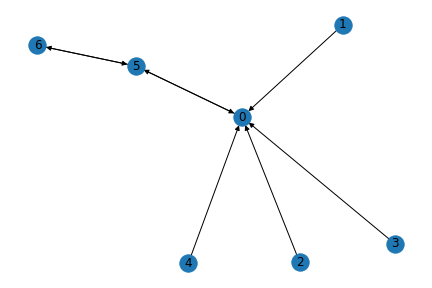
\includegraphics[width=0.55\linewidth]{figures/directed_graph_example_unranked.png}
  \caption{a weakly connected graph.}
  \label{fig:weaklyconnected}
\end{framed}
\end{figure}

In figure \ref{fig:weaklyconnectedpagedranked} we have the same
graph with vertex size and color indicating its PageRank with
parameter $\alpha=0.15$. We see that $5$ is ranked first, followed
by $0$. The smaller the restart parameter, the more important $5$
will get because we allow for longer paths with fewer restarts.

\begin{figure}[!htb]
\begin{framed}
  \centering
    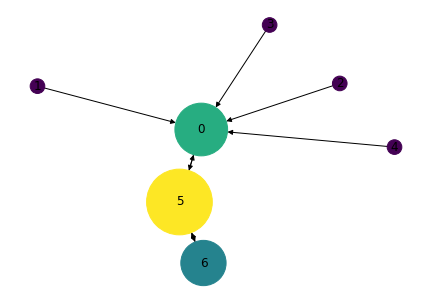
\includegraphics[width=0.55\linewidth]{figures/directed_graph_example.png}
  \caption{Pageranked graph.}
  \label{fig:weaklyconnectedpagedranked}
\end{framed}
\end{figure}

If we pick a restart parameter that is too large, which is the case
shown in figure \ref{fig:weaklyconnectedpagedrankedbadly}, the ranks
becomes almost uniform because the convex combination of the
original graph with the $n$-clique graph of the restarts is weighted
too heavily towards the latter. It also shows that for high restart
values $0$ becomes hotter than $5$. That is because paths of length
$\gt 2$ (before restart) become very unlikely in this random walk.

\begin{figure}[!htb]
\begin{framed}
  \centering
    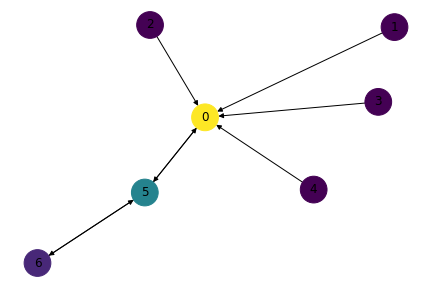
\includegraphics[width=0.55\linewidth]{figures/directed_graph_example_tinyalpha.png}
  \caption{again the same graph, with node color and size indicating
  their PageRank, with a restart probability approaching $1$.}
  \label{fig:weaklyconnectedpagedrankedbadly}
\end{framed}
\end{figure}

When we treat the same graph as undirected (figure
\ref{fig:undirectedanked} and calculate the PageRanks
($\alpha=0.15$), Vertex $0$ comes this time on top. It is more
central than $5$ and more random paths intersect it than any other
vertex.

\begin{figure}[!htb]
\begin{framed}
  \centering
    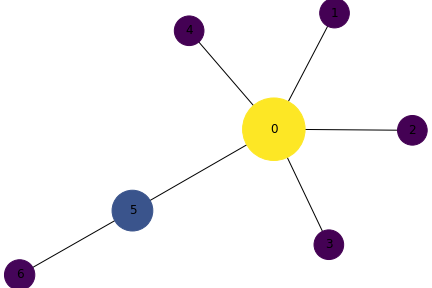
\includegraphics[width=0.55\linewidth]{figures/undirected_graph_example.png}
  \caption{same graph, but undirected.}
  \label{fig:undirectedanked}
\end{framed}
\end{figure}

In undirected graph, starts have hot centers and cold periphery.
a star has a hot center because it spreads its heat on many sources,
while each of the orbiting vertices sends all its heat into the star center.
The result is that hear accumulates at the center.

\begin{figure}[!htb]
\begin{framed}
\centering
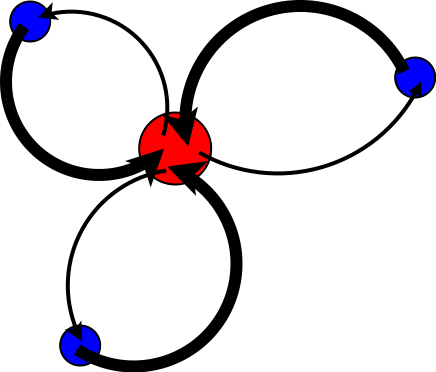
\includegraphics[width=0.55\linewidth]{figures/diagram_star.png}
\caption{a star graph.
}
\label{fig:hotstar}
\end{framed}
\end{figure}




%section
\newpage \section{A propagation based heuristic for graph clustering}

\subsection*{Prologue}
In this section we come up with a very simple simple clustering
heuristic algorithm which uses RWR to divide the well known Zachary's Karate
Club graph into 2 communities.
The original work tracks the splitting of a students karate club into 2 rivaling
clubs based on political and social affiliations.
The results of the algorithm are compared to the actual
social structure.

\subsection*{Theory}

\begin{mydef}
\label{def:influence}
Let $G$ be a strongly connected graph and $K$ the diffusion matrix as defined in
\ref{lem:invertible}, end let $u,v \in \{1 \dots n\}$ be two vertices and $e_u,
e_v \in \R^n$ their corresponding index vectors.

$p_u := K e_u$, the stationary distribution with random restart from $u$,
is called the \textbf{influence vector} of vertex $u$. We say that
$p_u[v] = K[v,u]$
is the \textbf{influence of} $u$ on $v$. In terms of random walk,
$K[v,u]$ is the frequency that we visit $v$, if we do a RWR from
$u$. 
\end{mydef}

\begin{remark}
\label{rem:influence}
We use the definition of influence as presented in the Hotnet and
Hotnet2 artticles \cite{vandin2012discovery} and
\cite{leiserson2015pan}.

Remember that we use in this paper $A \cdot v$ scheme while
because that is the 'normal' way in linear algebra textbooks.
However often in papers dealing with Markovian processes they use
the other way. To add to the confusion, they sometime call these conventions
left (repectively right) multiplication but whose left and whose
right and why?
\end{remark}

A $p_u$ is a measure of how 'heat' which is pumped into $u$ propagates in the graph.
When we try to cluster the graph, it is natural to think that If vertex $v$
is the top receiver from $u$, namely $v = \text{argmax}(p_u)$ then maybe these 2
belong in the same cluster.

Informally we say that a vertex is 'hot' or 'cold' if it has a high (hot) or low
(cold) PageRank. Remember that the PageRank is the unbiased stationary distribution
$p = K \cdot (1/n, \dots, 1/n)^t$.

We suggest that it makes sense to pick up a
cold vertex and associate it with the vertex to which it sends most of its heat.
If we start from a hot vertex, it usually has many neighbours and it doesn't
send allot of heat down a single vertex.

The algorithm works as follows:

\begin{lstlisting}
function coolWarmClustering(G, k)
  # Input G = (V,E) : a directed strongly connected graph.
  # Input m : The desired number of clusters
  K <- diffusion_kernel(G)
  # each vertex starts in its own cluster: 
  H <- Disconnected_undirected_graph_on(V) 
  p <- pageRank(G)
  # vertex-list sorted up by PageRank: 
  vlist <- arg_sort(p)
  While |connected_components(H)| > k do
    # take the coldest remaining vertex 
    # and remove it from the list:
    x <- vlist.pop()
    # Influence vector of x:
    p_x <-K * e_x 
    # find the max excluding the already visited nodes 
    y <- argmax(p_x[i : i in vlist])
    H.add_edge(x,y)
  return H
\end{lstlisting}

The algorithm clusters the vertices by constructing a new graph on the same
vertices, successively joining vertices. It picks the coldest remaining vertex
and joins it with the vertex to which it propagates the most heat, among
the yet unvisited vertices.

In every iteration of the algorithm adds an edge from the currently
selected vertex to one of the remaining vertices which haven't been
selected yet.The
number of connected components by $1$. Because $G$ is
strongly connected the algorithm will reduce the number of connected
components in $H$ until it reaches the desired number of components
$k$.

It is essential to run the algorith in the order from lower pageranked
vertices upwards. If we start for example the other way around, from
the warmest node downwards, the list of remaining nodes contains the
coldest and least 'relevant' nodes.

\begin{figure}
\begin{framed}
\centering
\begin{subfigure}[b]{0.5\textwidth}
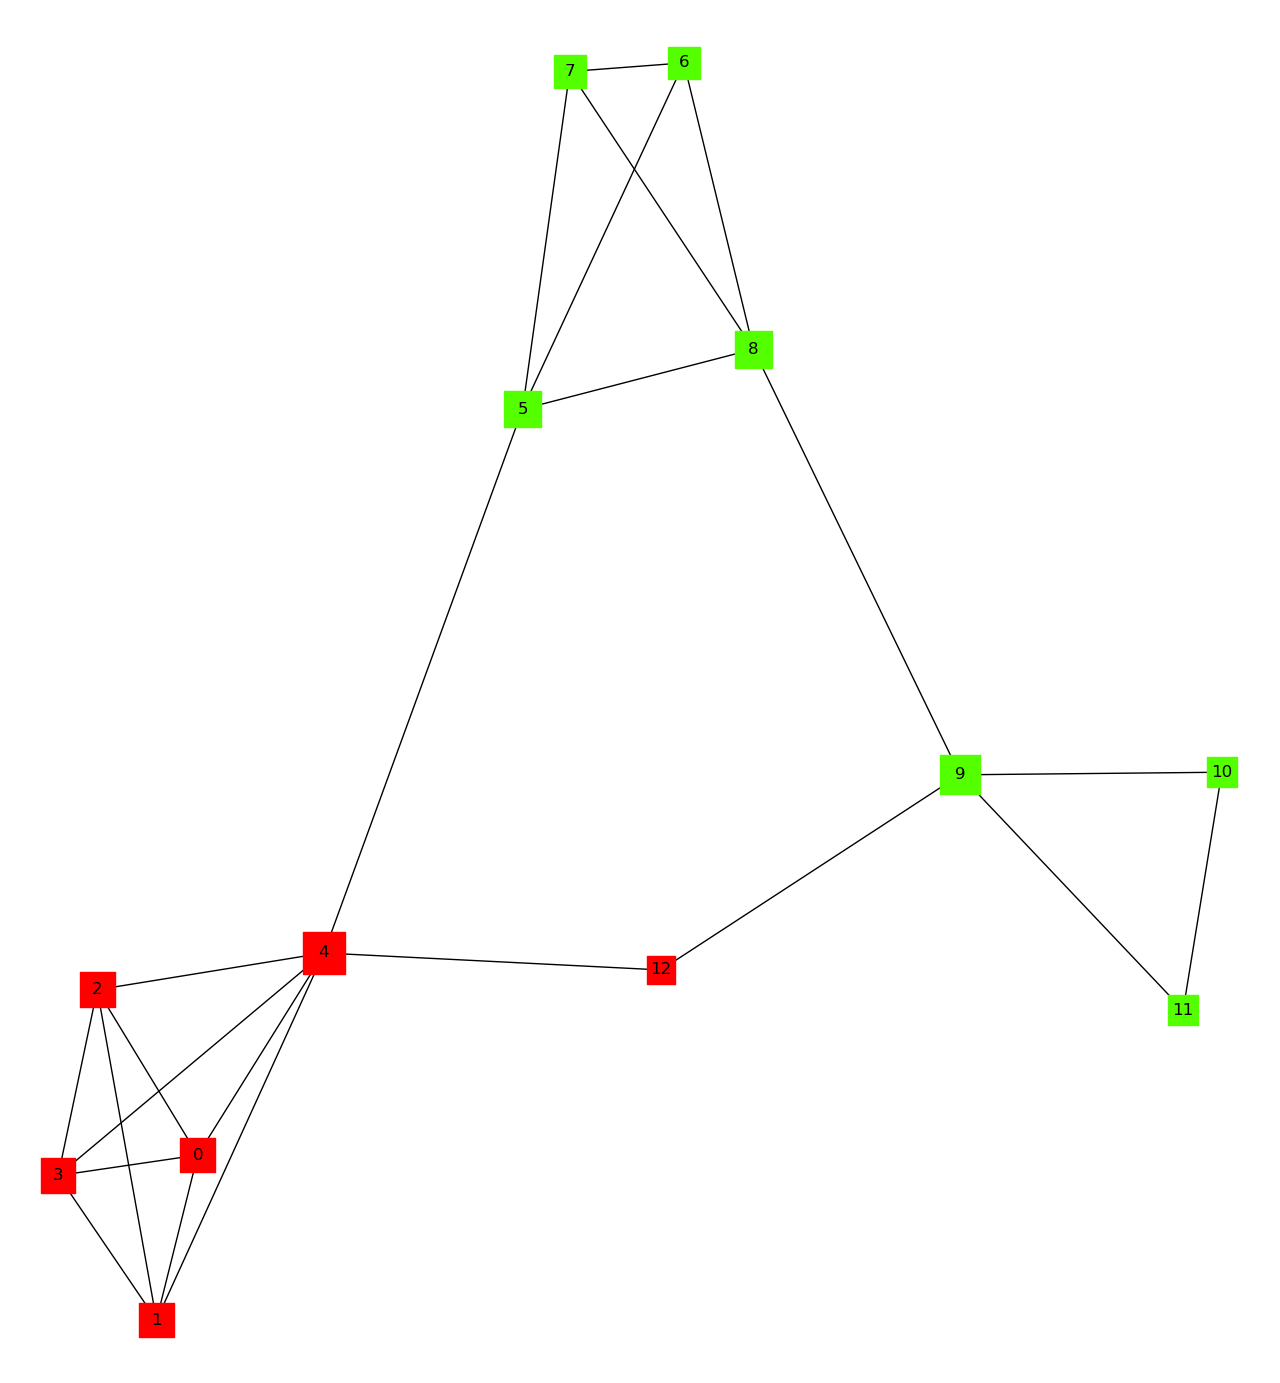
\includegraphics[width=\textwidth]{figures/example_coolwarm2clusters.png}
\caption{A 2 cluster partition}
\label{fig:examplecoolwarm2cluster}
\end{subfigure}
%add desired spacing between images, e. g. ~, \quad, \qquad, \hfill etc. 
%(or a blank line to force the subfigure onto a new line)
\begin{subfigure}[b]{0.5\textwidth}
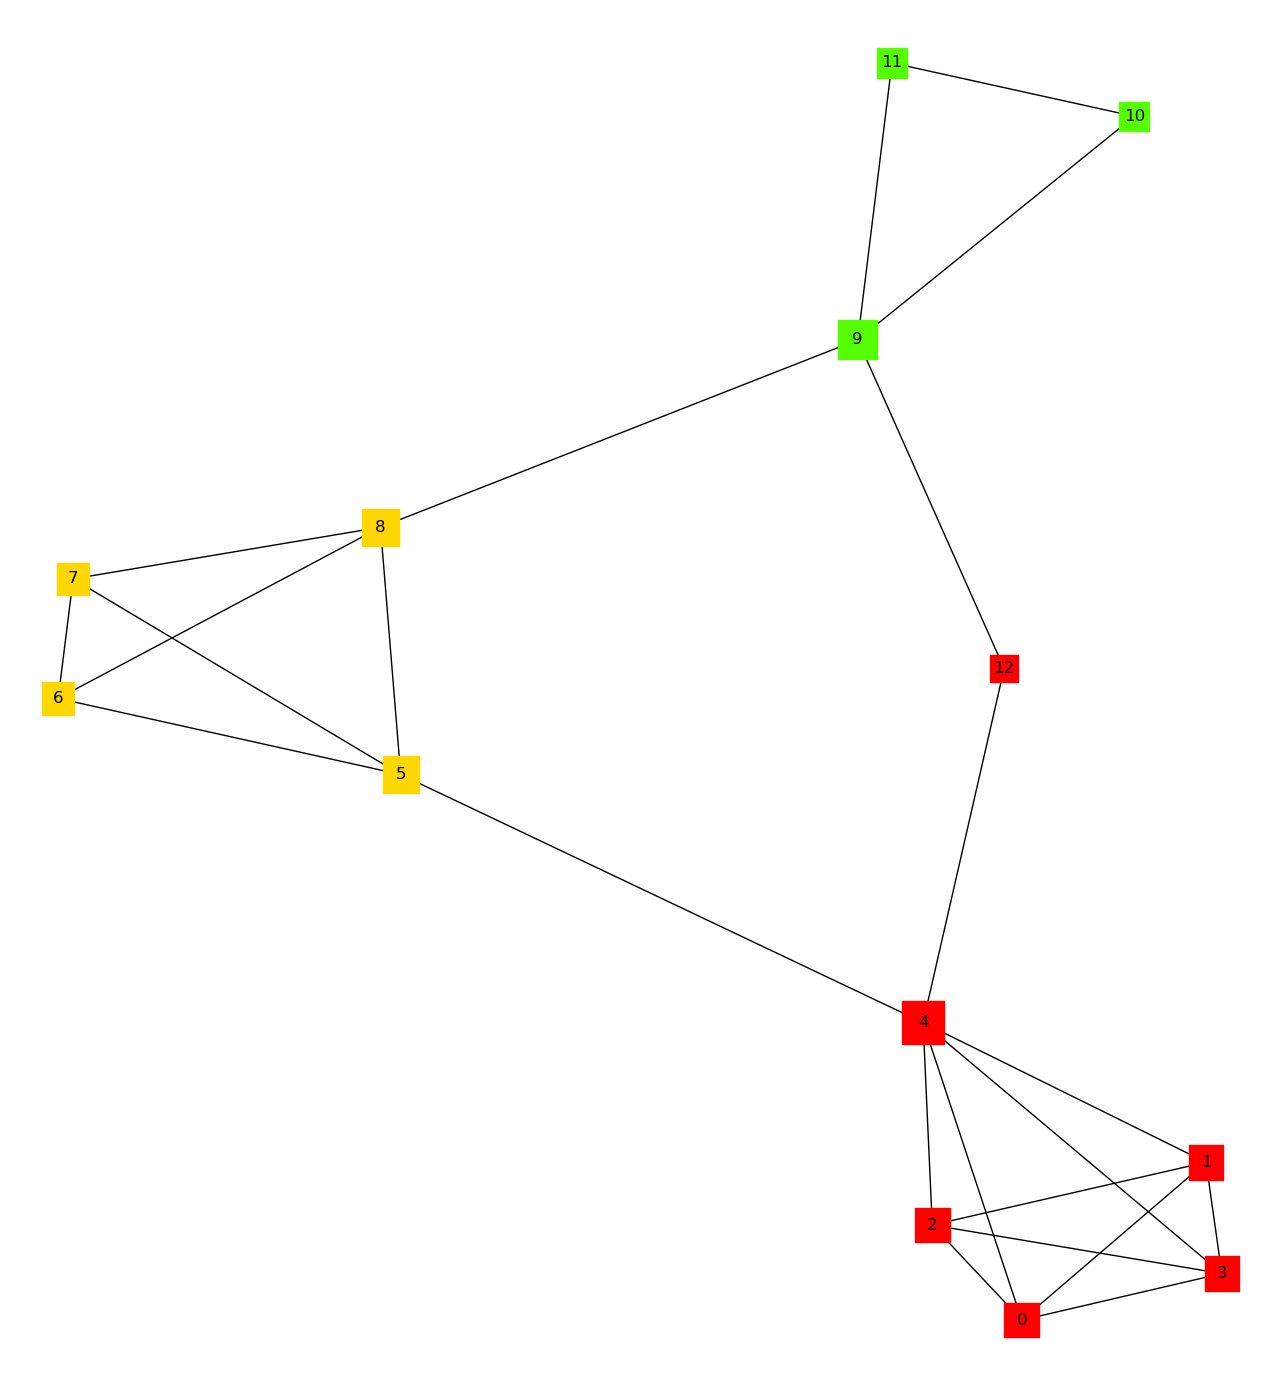
\includegraphics[width=\textwidth]{figures/example_coolwarm3clusters.png}
\caption{A 3 cluster partition}
\label{fig:examplecoolwarm3cluster}
\end{subfigure}
%add desired spacing between images, e. g. ~, \quad, \qquad, \hfill etc. 
%(or a blank line to force the subfigure onto a new line)
\caption{'toy graph' used for testing the algorithm}
\label{fig:exampleCoolWarmClustering}
\end{framed}
\end{figure}

\subsection*{Testing of the algorithm}

We tested the algorithm on a small 'toy graph', as well as on the
famous 'Zachary's Karate Club' graph. In the appendix C, which deals
with spectral clustering, we a tested a basic spectral clustering 
method on the same graphs.

Figures \ref{fig:exampleCoolWarmClustering} are showing the results
of running the algorithm set for finding a 2-partition and
respectively a 3-partition on a 'toy graph'. The interesting node is
12. In both runs 12 chooses to associate with the biggest clique
because node 4 of that clique is the one which receives the most
heat from 12

\begin{figure}[!htb]
\begin{framed}
\centering
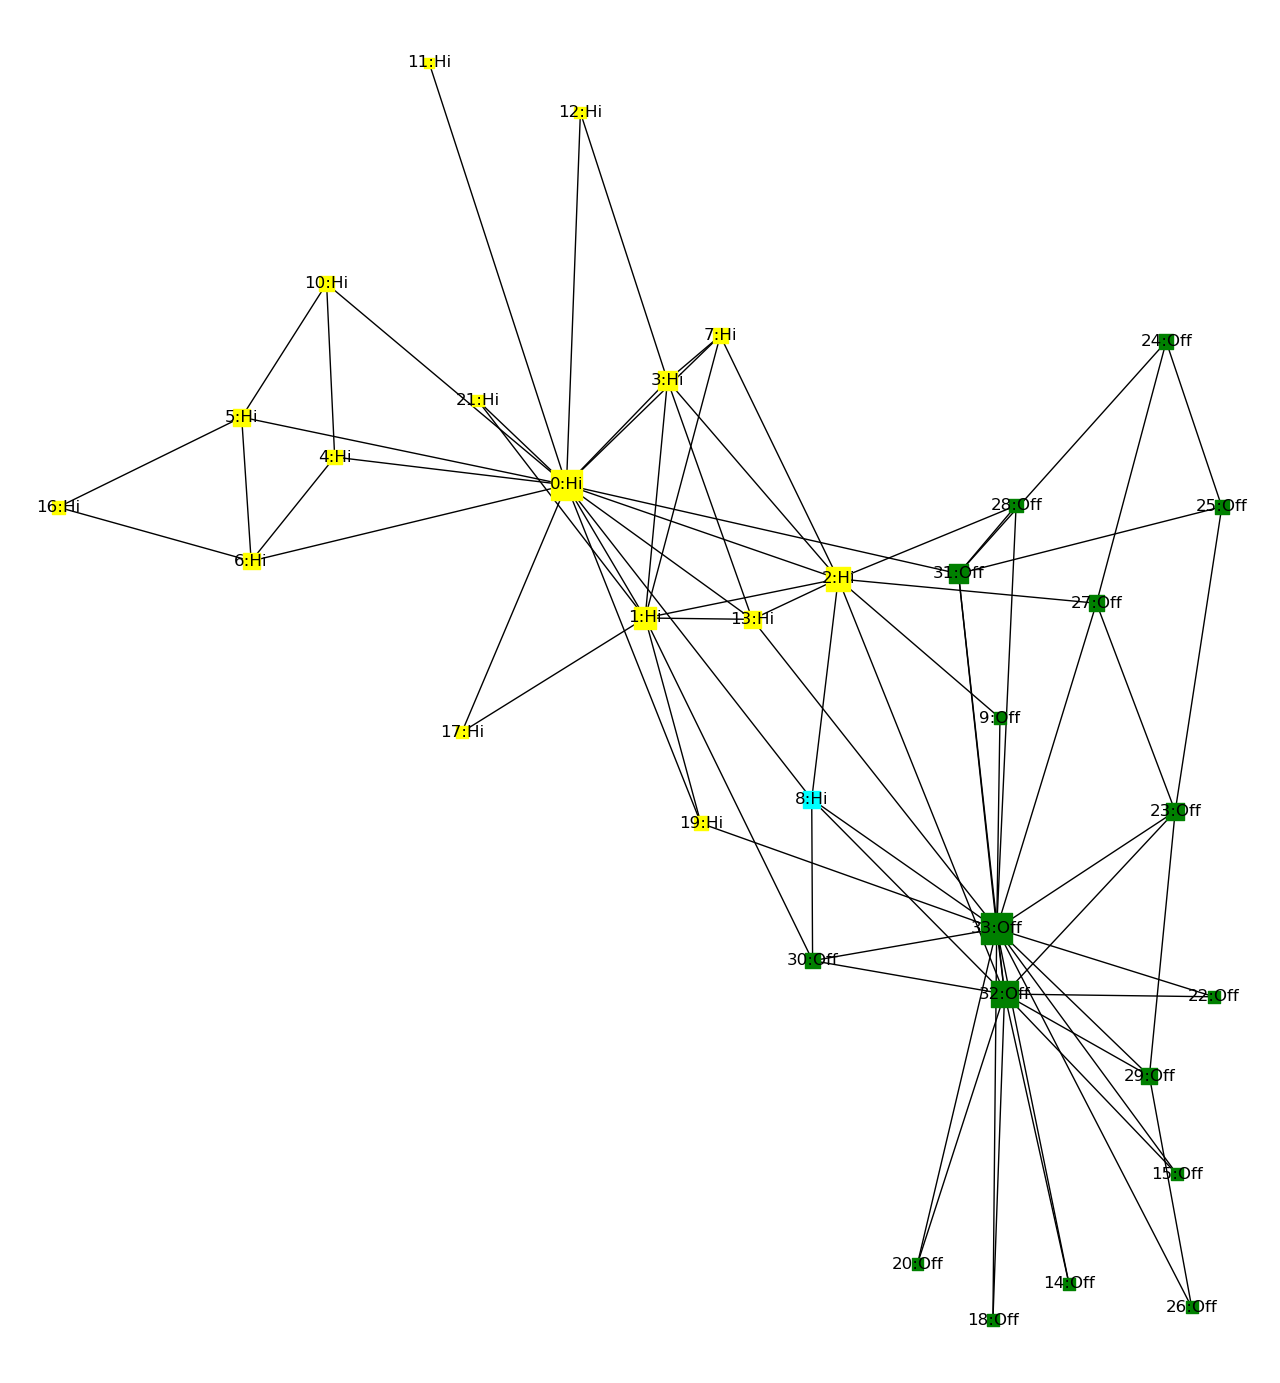
\includegraphics[width=0.97\linewidth]{figures/Karate_coolwarmclustering.png}
\caption{
'Zachary's Karate Club'.
'Mr Hi' (Yellow) and 'Officer' (Green) groups.
The Cyan colored node indicates a mismatch between the clustering
and the actual division.
}
\label{fig:karatecoolwarm}
\end{framed}
\end{figure}

Figure \ref{fig:karatecoolwarm} shows the results of running the
algorithm on the 
famous 'Zachary's Karate Club' Graph. The labels show the actual division
between the 'Mr Hi' and 'Officer' groups.
Vertex size indicates its PageRank.
The colors encode the result of the coolWarmClustering compared to the actual
partition. Yellow indicates true positive for 'Mr Hi', green is a
true positive for 'Officer', and cyan is a mismatch between
the clustering algorithm and the actual division.
There is only one mistake:
It associates wrongly vertex 8 to 'Officer'.  This vertex
is hard to resolve because it is connected to hubs in both clusters.
In fact a further check confirms that the total sum of 'heat' it sends to members of
'Officer' is $0.45$ vs $0.36$ to members of 'Mr Hi' (excluding itself in both
cases). So in some sense the algorithm is more correct then the actual
partition in real life. Perhaps this is due to human irrationality?
On the other hand, vertex $8$ receives more heat units from $17$ members of 'Mr. Hi': $0.485$
units, compared to $0.345$ units from the $16$ members of 'Officer'. 




%section
\newpage %\usepackage{listings}
\section{A function prediction method}
\subsection*{Prologue}
As we mentioned in the introduction our main goal was to develop
a classification algorithm for the PLC problem which can be used for the
purpose of protein function prediction in a partially annotated PPI
network.

What it means is we are going to take an input a strongly connected
graph where the vertices represent protein types and the edges represent
observed interaction between them. The some of the proteins are
annotated with a label that specifies their function. The rest are
unannotated.

The prediction algorithm outputs a suggested label for each unlabeled protein.
Our paradigm is that protein is that proteins of the
same label should form, approximately, a community in the sense of
graph community structure which we discussed in the earlier sections.
Since the algorithm is using propagation methods which are closely
related to the community structure of the graph, if the paradigm doesn't
hold then the prediction sohould be no better than a coin toss.

It is understood that proteins that interact more likely than not
share the same function~\cite{schwikowski2000network}. It's a weaker
property than our paradigm because it doesn't speak about communities,
only about adjacent proteins.

The diffusion matrix provides us with ranking such that for for every
vertex $i$ we can weigh the other vertices by 'importance' to that
vertice (namely it's the $i$ row of the diffusion matrix). We use that
information to predict the label of the protein. We assume that members
of the same label of the protein will have cumulatively the most
'influence' on it. We also assume that the distribution of labeled and
unlabeled is the same across the network so by removing them from
consideration, still the proteins that share the same label with the
protein we test will have the most cumulative influence on it.

We tested and compared 5 different methods, 3 were diffusion based and 2
were neighbor based which we used mainly as the reference point.

The source code for all the algorithms and the test can be found at
the project's git repository~\cite{project_git}.

\subsection*{The Algorithm}

We tried 5 different prediction methods:

\begin{itemize}
\item{Method 1} Determines the group affiliation of an unknown node
by the group that has the maximal volume based on the propagation
distribution from the unknown node. This meas: we calculate the
stationary distribution with restart to the unknown node. Among the
known nodes, we calculate the weighted sums of each of the 4 groups
according to that distribution. The group with largest volume (see
pseudo code for the decision function below) is the affiliation we
assign to the unknown node.


\item{Method 2} This method works like method 1, except that we first order the
unknown nodes according to their pageRank. We go over the
nodes in this order and assign group affiliation according to method 1, but then
we also update the list of the known nodes to include that node. So this node is
going to be included in the function prediction of the lower ranked nodes.

The rational here was that the RWR as we have seen has the property
that heat flows from the low ranks to the high ranks. So maybe we
should pick a low ranked vertex and see where it flows to.
If we start from a hot central vertex.

\item{Method 3} We assign an unknown node to the group that has plurality among
its neighbors with known group affiliation. So this method is fast and
probably the simplest. This method is essentially the 'prediction
function' from \cite{schwikowski2000network}.

\item{Method 4} Same as method 3, but again we go in the order of pagRanks and
we update the list of known nodes on the fly, like method 2.

\item{Method 5} Here we take each group of the known nodes and propagate from
it. So for example we calculate the stationary distribution when we restart in
the known nodes that belong to group 'DNA Replication', and then for the next
group and so forth. For each unknown node, we assign it to the group that
propagates the highest probability to it.

While in method 1 and 2 we start random walking from an unknown node and see
what is the probability that we land at a certain group, In Method 5 we start
walking randomly from one of the members of a group and check what is the
probability that we visit a certain unknown node.

This method is an order of magnitude faster than method 1 and 2 because we only
need to calculate the stationary distributions 4 times (pageRank and for each
group). However we suspect it will perform with less accuracy.
The reason for that is that method 5 takes into account nodes that are far and not well connected to the
unknown node whose function we try to predict.
The function groups, in particular the yellow (meiosis) and green (stress) are not
well clustered and spread all over the network but we can see that
some subsets of these labels form clusters.

\end{itemize}

\begin{minipage}{\linewidth}
\begin{lstlisting}[mathescape=true, 
    caption = {method 2, decision funciton}, label={code:decision_function}]
# vertices are enumerated 1 to n. labels are enumerated 1 to m.
# input v: vertex of unknown label, to be predicted
# input F: the diffusion matrix (so F is column-normalized)
# input labeledSubset: list of boolean vectors. so
#    if labeledSubset[l] = (1, 0, ...),
#    then vertex 1 has label l and vertex 2 doesn't.

def decisionFunction(v, F, labeledSubset):
  # get p, the influence vector of v, which is column v of F:
  let $p$ = $F \cdot e_v$
  let labeledSums = [sum(p[x]) for x in labeledSubset]
  return argmax(labeledSums)
\end{lstlisting}
\end{minipage}

\begin{minipage}{\linewidth}
\begin{lstlisting}[mathescape=true, 
    caption = {method 2, main funciton}, label={code:method2}]
# vertices are enumerated 1 to n. labels are enumerated 1 to m.
# Input G: a strongly connected graph
# input labeledSubset: list of boolean vectors. so 
#    if labeledSubset[l] = (1, 0, ...),
#    then vertex 1 has label l and vertex 2 doesn't.

def predictionMethod2(G, labeledSubset):
  # calculate the diffusion matrix
  let F = diffusionMatrix(G)
  # calculate the pageRank order
  let pr = $F \cdot \bar{1}/n$
  let unknowOrderedList = [v : v is unlabeled].sort_up_by(pr)
  for v in unknowOrderedList:
    predLabel <- decisionFunction(v,F,labeledSubset)
    # set v's labels to predLabel
    # it will participate in the subsequent predictions
    labeledSubset[predLabel][v] <- 1
  return labeledSubset
\end{lstlisting}
%this is listing \ref{code:decision_function}.
\end{minipage}

\subsection*{Experimental Protocol}
We first constructed a \textbf{fully} labeled subnetwork of the
yeast interactome by choosing arbitrarily 4 labels, the only
constrain was that each labeled subset be sufficiently large (approximately
100 or more nodes).
We then removed from the network all nodes that didn't have one of
those 4 labels: 'DNA replication' (blue), 'Golgi' (red), 'Meiosis'
(yellow), and 'Stress response' (green). We also removed nodes that
had more than one of these 4 labels (of which there were only a
handful). The resulting subnetwork is shown in figure
\ref{fig:yeast_subgraph_4groups}. 
We then selected the greatest connected component of that network,
and this was our experimental graph.
It contains around 500 vertices.

In the first set of tests, we tested the accuracy of each of the 5
methods. We randomly selected 50\% of the nodes and
assigned them to the known group, that is, they were the labeled
subset. The rest were the unlabeled. We ran each of the 5 methods on
this partially labeled networked and validated its accuracy by
comparing its prediction with the fully labeled network. We repeated
these tests twice, on 2 different randomly selected labeled subsets.
The results are in table~\ref{table:results_5_prediction_methods}

We then chose method 2 which had the highest accuracy for further
tests. We tested it with different parameters, repeating each
settings 50 times with 50 different sets of known labels. The
parameters we tested were the restart probability ($\alpha$) and
what we called the \textbf{labeled coverage}, which is the portion
of the nodes that start with a known label.

We have conducted another test of method 2, with parameters $\alpha
= 0.31$, and label coverage of $0.35$. This time we calculated the
sensitivity, specificity, accuracy and precision (PPV) for each
label as well as the total.

\begin{figure}[!htb]
\begin{framed}
\centering
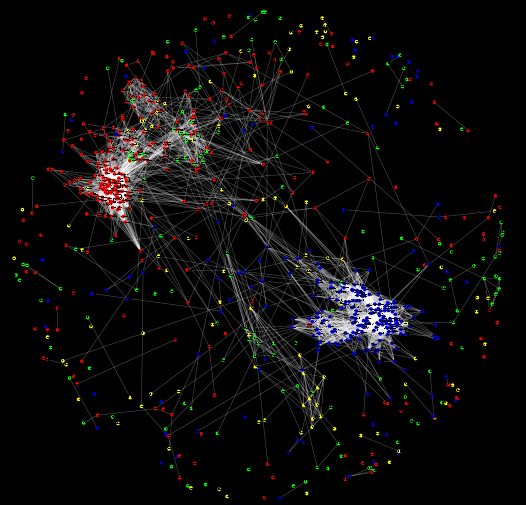
\includegraphics[width=\textwidth]{figures/yeastsubgraph_4_groups_colorcode.png}
\caption{Subgraph of the yeast interactome showing nodes of 4 groups: 'DNA
replication' (blue), 'Golgi' (red), 'Meiosis' (yellow), 'Stress response'
(green)}
\label{fig:yeast_subgraph_4groups}
\end{framed}
\end{figure}

\subsection*{Results}

Table~\ref{table:results_5_prediction_methods} shows the results of
the experimentally measured accuracy for each of the 5 method on 2
50\% labeled networks (the networks are the same, the labeled
vertices were randomly selected). 

\begin{table}[!htb]
\caption{Prediction Accuracy of the 4 Methods in 2 different random
trials. Each trial with a different seed, which result in different randomly
selected known/unknown nodes.} 
\begin{center}
\begin{tabular}{ | l | c | c | c | c | c | }
\hline
Seed / Method & 1 & 2 & 3 & 4 & 5\\
\hline
42 & 0.795 & 0.854 & 0.765 &
0.791 & 0.701\\
6382020 & 0.774 & 0.832 & 0.751 & 0.751 & 0.755\\
\hline
\end{tabular}
\label{table:results_5_prediction_methods}
\end{center}
\end{table}

We picked method 2 which was the best performer for further tests.
Figure~\ref{fig:largest_connected_comp}
shows the network and the hits and misses of the prediction
algorithm method 2.

\begin{figure}[!htb]
\begin{framed}
\centering
\begin{subfigure}[b]{\textwidth}
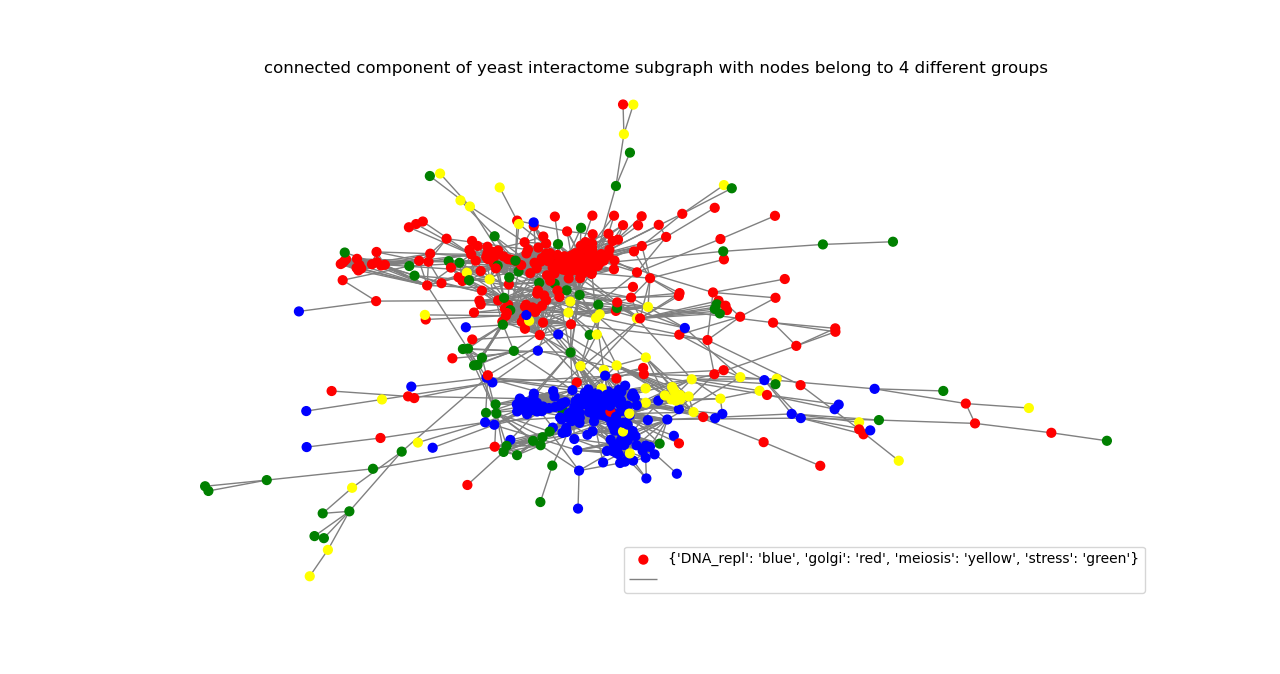
\includegraphics[width=\textwidth]{figures/connected component of yeast interactome subgraph with nodes belong to 4 different groups.png}
\caption{The largest connected component which was selected for the function
prediction experiment. Here the Correct group affiliation of all nodes is color
coded.}
\end{subfigure}
\begin{subfigure}[b]{\textwidth}
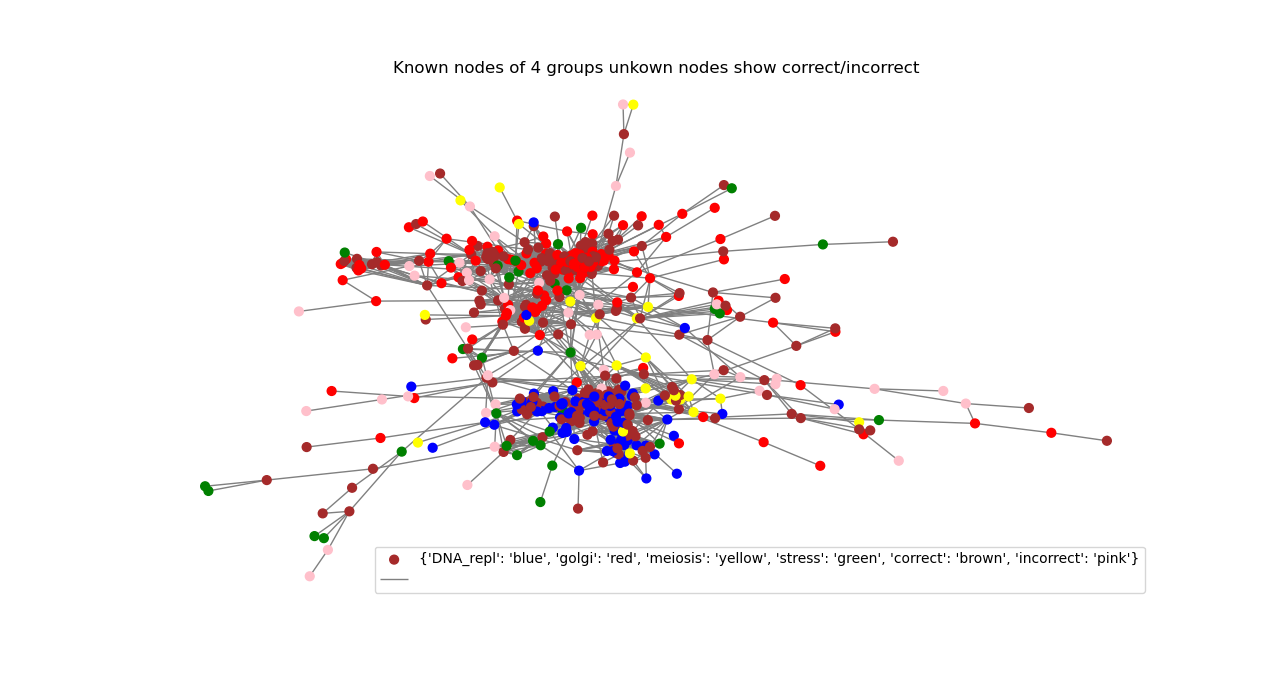
\includegraphics[width=\textwidth]{figures/method2_true_false_clustering_on_4_groups_with_ordering_and_update.png}
\caption{The result of predictiob method 2, which was the best perfomer. 
The known groups are color coded by RGBY. The unkown nodes are color
coded: brown:correct prediction, pink:incorrect.}
\label{fig:my_prediction}
\end{subfigure}
\caption{The test network}
\label{fig:largest_connected_comp}
\end{framed}
\end{figure}

Upon further testing we conducted with method 2,
the best mean result (for coverage of 0.5), was $0.8926$ mean accuracy.
It was obtained with a
restart probability of $0.31$. Restart parameters $\alpha \in [0.2-0.3]5$, lets
call it mid-lower range, produce the best results, while with higher
alphas accuracy falls towards $0.5$ which is of course the accuracy of
just randomly guessing. 

Accuracy was about 0.8 when we start with only 10\% labeled and it
gradually increases with increased labeled proportions (0.85 accuracy at
0.3 label coverage). We plotted the relationship between accuracy and
the parameters in figure \ref{fig:alpha_fracs}.

\begin{minipage}{\linewidth}
We have tested method 2 for accuracy, precision, specificity and
sensitivity, with parameters $\alpha = 0.31$, and label coverage of
$0.35$. The values were calculated for each label as well as the
total. The results are the following:

\begin{lstlisting}[basicstyle=\footnotesize, label=tab:sens]
      Label      P     TP    FP        N       TN    FN Sens Spec  Acc  PPV
0     golgi    165    149    25      209      184    16 0.90 0.88 0.89 0.86
1  DNA_repl    133    129    22      241      219     4 0.97 0.91 0.93 0.85
2   meiosis     30     17     4      344      340    13 0.57 0.99 0.95 0.81
3    stress     46     25     3      328      325    21 0.54 0.99 0.94 0.89
4     Total 374.00 320.00 54.00 1,122.00 1,068.00 54.00 0.86 0.95 0.93 0.86
\end{lstlisting}
\label{tab:senspec}

We can see that the problem lies with the two small and spread out
groups, 'meiosis' and 'stress'. It is hard to predict that an
unlabeled vertex belong to these groups 

\end{minipage}

\begin{figure}[!htb]
\begin{framed}
\centering
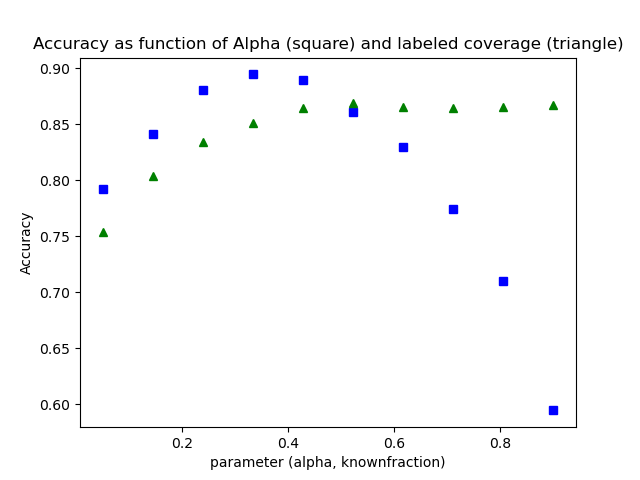
\includegraphics[width=\textwidth]{figures/alpha_fraq_graph.png}
\caption{The accuracy as function of the resart parameter alpha,
with fixed label coverage of 0.5, and of the label coverage with
fixed alpha=0.2}
\label{fig:alpha_fracs}
\end{framed}
\end{figure}

\subsection*{Remarks and Conclusions}

If we look at figure \ref{fig:largest_connected_comp} which shows the connected
component that we worked with, the red and blue are pretty nicely clustered. The
greens and specially the yellows are sort of spread all over the network and
not nicely clustered. We don't know if this is a good example of a real world
scenario in the context of PPI networks.

When we look at figure \ref{fig:my_prediction} it seems that most of the
incorrect predictions are on nodes that seem 'peripheral' and  are not well
connected to known nodes. Another source of mistakes seems to bee green nodes
that are too close to the red cluster.

Method 2 shows somewhat higher accuracy over the other methods but on the flip
side it is an $O(n^2)$ method when optimized methods are used whereas methods
3,4,5 are $O(n)$.

We suspect (but it requires testing) that the accuracy of methods 3
and 4 would decrease more rapidly with decreasing labeled coverage
than it did with method 2. The reason is that methods 3 and 4 become
completely arbitrary on a vertex which has no labeled neighbors.
Method 1,2 rank all the vertices on a graph so they may have a
better chance of finding the right label. 



%Section 4 gave us a strong indication about the usefulness of the
%diffusion matrix as as a type of quasi-distance with which we
%measure closeness or 'influence' between nodes in the network.
%Our working paradigm is that connected nodes are more likely to have
%the same functional class than not, a fact which has been shown to
%be true by \textcite{schwikowski2000network}.
%
%In this section we are going to apply the accumulated knowledge of the
%previous sections and devise some simple function prediction algorithms for PPI
%networks. We to try several methods which use propagation as well as
%methods which just use direct neighbors for the predictions.
%
%The network is going to be composed of around 500 vertices (proteins) which are
%divided into 4 different function groups. We are going to randomly choose half
%the proteins and mark them as unknown and try to predict their function based
%on the remaining known proteins. Then we can verify the results with the
%actual annotations.

%\subsection{Tools and Source Data}
%
%We sourced our data from \textcite{cytoscape}, an open source
%java software for network analysis and visualisation. 
%The software as one of its built in examples a
%fully annotated yeast interactome. This is a PPI network of
%thousands of proteins and it contains among many other types of
%edge and node annotations information about protein function and
%location in the 'MCs name' field.
%
%We preferred to work within the familiar Python 3 programming
%language and its rich world of extension libraries and packages.
%Therefore we exported the yeast interactome into a graphml format
%which was later imported into our network analysis tool of choice,
%\textcite{networkx}. This is a python based open sourced network analysis 
%package which integrates extremely well with other essential Python
%packages. Networkx is neither as versatile nor as powerful as Cytoscape and
%especially rudimentary in its visualisation functionality, but it
%runs smoothly and is easy to work with, unlike Cytoscape.
%We used the \textcite{numpy} package for vector, matrix and other
%types mathematical
%calculations, and \textcite{pandas} for some database operations. 
%
%\subsection{Methodology}
%As mentioned, we 
%used the annotated yeast interactome which is a pure PPI network that comes
%prepackaged with the
%software tool 'Cytoscape'. The nodes represent yeast proteins and the edges
%represent protein-protein interactions.
%
%This network comes with functional annotations in the 'MCs name' field.
%We selected nodes in the network whose annotations contain
%\textbf{exactly} one of the following keywords:  'DNA Replication' (blue
%group), 'Golgi' (red), 'Meiosis' (yellow), and 'Stress response'
%(green). All other nodes are removed from the network.  The result is
%shown in figure \ref{fig:yeast_subgraph_4groups}.
%
%The resulting subnetwork is not a connected graph, which is the type
%of input data that we wanted to run our test algorithm on. Therefore
%we selected the biggest connected component of that subnetwork, and
%that is the graph on which we tested and compared various prediction
%algorithms.
%
%
%For the first set of comparative tests of different prediction
%methods 
%we set a random seed (a process which we repeat 2 times for 2 different trials).
%Then we selected randomly 50\% of the nodes and marked them as 'unknown'. The other
%50\% are 'known'. We would then try to determine the group affiliation of the
%unknown nodes based on the group affiliations of the known nodes.

%We tried 5 different prediction methods:
%
%\begin{itemize}
%\item{Method 1} Determines the group affiliation of an unknown node by the group
%that has the maximal volume based on the propagation distribution from the
%unknown node. This meas: we calculate the stationary distribution with restart
%to the unknown node. Among the known nodes, we calculate the weighted sums of
%each of the 4 groups according to that distribution. The group with largest
%volume is the affiliation we assign to the unknown node.
%
%\item{Method 2} This method works like method 1, except that we first order the
%unknown nodes (decreasing order) according to their pageRank. We go over the
%nodes in this order and assign group affiliation according to method 1, but then
%we also update the list of the known nodes to include that node. So this node is
%going to be included in the function prediction of the lower ranked nodes.
%
%The rational here is that the higher ranked nodes are probably going to be
%predicted with high accuracy and therefore be helpful in prediction of lower
%ranked nodes. 
%
%It is probably better to device some simple rule to decide whether it is worth
%to include a node in the prediction of the rest of the nodes. For example, based
%on how many unknown neighbors in has vs known neighbors. But we tried to keep
%things simple at this stage.
%
%\item{Method 3} We assign an unknown node to the group that has plurality among
%its neighbors with known group affiliation. So this method is fast and
%probably the simplest.
%
%\item{Method 4} Same as method 3, but again we go in the order of pagRanks and
%we update the list of known nodes on the fly, like method 2.
%
%\item{Method 5} Here we take each group of the known nodes and propagate from
%it. So for example we calculate the stationary distribution when we restart in
%the known nodes that belong to group 'DNA Replication', and then for the next
%group and so forth. For each unknown node, we assign it to the group that
%propagates the highest probability to it.
%
%While in method 1 and 2 we start random walking from an unknown node and see
%what is the probability that we land at a certain group, In Method 5 we start
%walking randomly from one of the members of a group and check what is the
%probability that we visit a certain unknown node.
%
%This method is an order of magnitude faster than method 1 and 2 because we only
%need to calculate the stationary distributions 4 time (pageRank and for each
%group). However we suspect it will perform with less accuracy.
%The reason for that is that method 5 takes into account nodes that are far and not well connected to the
%unknown node whose function we try to predict.
%The function groups, in particular the yellow (meiosis) and green (stress) are not
%well clustered and spread all over the network but we can see that
%some subsets of these labels form clusters.
%
%\end{itemize}


%\subsection{Results}

%\begin{table}[!htb]
%\caption{Prediction Accuracy of the 4 Methods in 2 different random
%trials. Each trial with a different seed, which result in different randomly
%selected known/unknown nodes.} 
%\begin{center}
%\begin{tabular}{ | l | c | c | c | c | c | }
%\hline
%Seed / Method & 1 & 2 & 3 & 4 & 5\\
%\hline
%42 & 0.795 & 0.854 & 0.765 &
%0.791 & 0.701\\
%6382020 & 0.774 & 0.832 & 0.751 & 0.751 & 0.755\\
%\hline
%\end{tabular}
%\label{table:results_5_prediction_methods}
%\end{center}
%\end{table}

%We decided to further experiment with method 2.
%We tested it with different parameters, repeating each settings 50 times
%with 50 different sets of known labels. The parameters we tested were
%the restart probability ($\alpha$) and what we called the labeled
%coverage, which is the portion of the nodes that start with a known
%label.
%The best mean result (for coverage of 0.5), was $0.8926$ mean accuracy.
%It was obtained with a
%restart probability of $0.31$. Restart parameters $\alpha \in [0.2-0.3]5$, lets
%call it mid-lower range, produce the best results, while with higher
%alphas accuracy falls towards $0.5$ which is of course the accuracy of
%just randomly guessing. 
%
%Accuracy was about 0.8 when we start with only 10\% labeled and it
%gradually increases with increased labeled proportions (0.85 accuracy at
%0.3 label coverage). We plotted the relationship between accuracy and
%the parameters in figure \ref{fig:alpha_fracs}.
%
%\begin{figure}
%\begin{framed}
%\centering
%\begin{subfigure}[b]{\textwidth}
%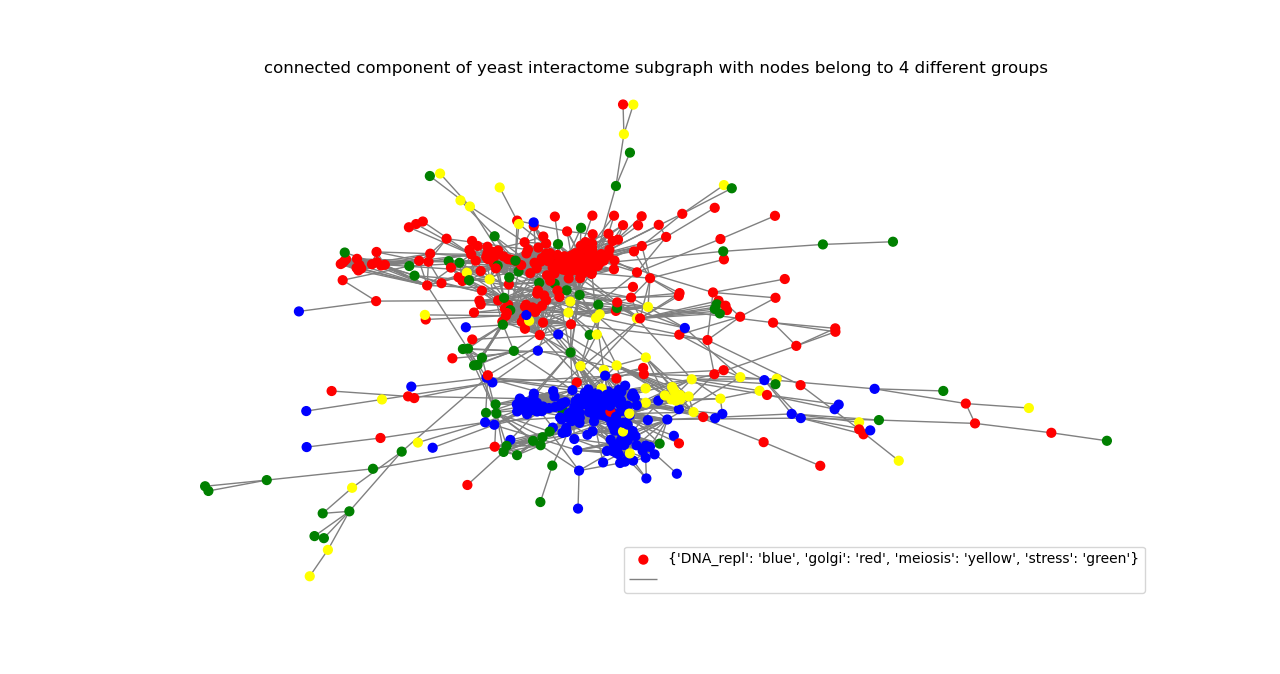
\includegraphics[width=\textwidth]{figures/connected component of yeast interactome subgraph with nodes belong to 4 different groups.png}
%\caption{The largest connected component which was selected for the function
%prediction experiment. Here the Correct group affiliation of all nodes is color
%coded.}
%\label{fig:largest_connected_comp}
%\end{subfigure}
%\begin{subfigure}[b]{\textwidth}
%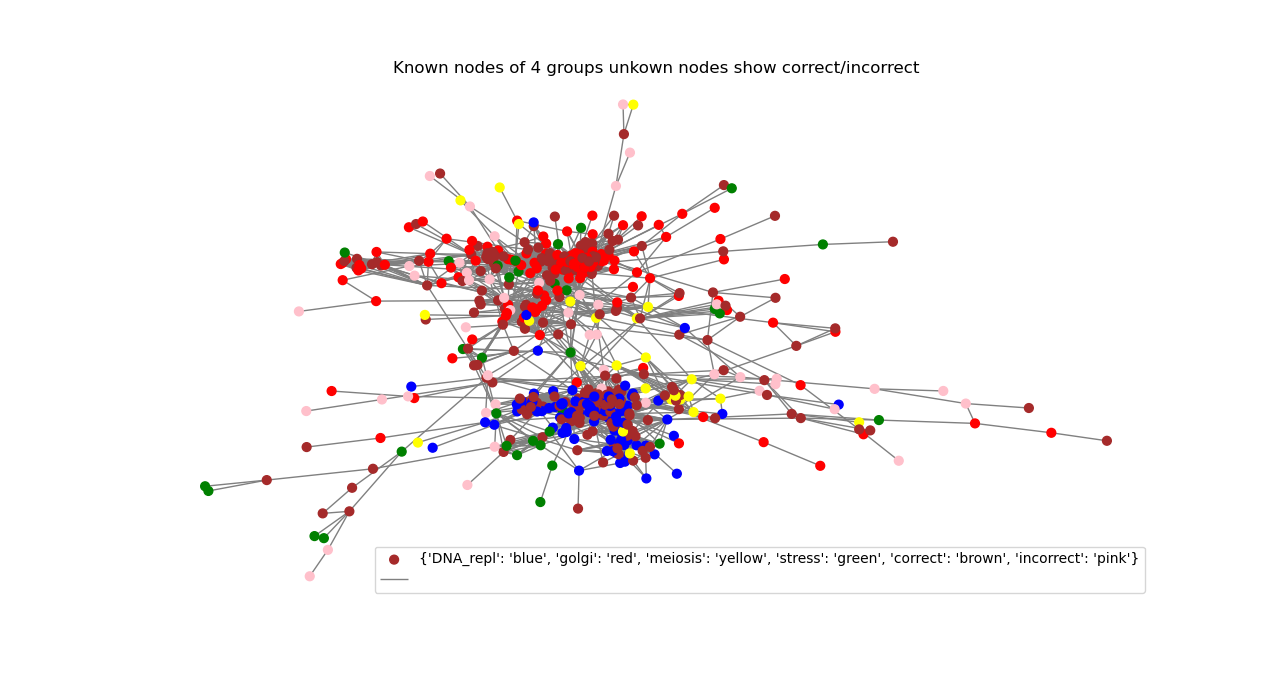
\includegraphics[width=\textwidth]{figures/method2_true_false_clustering_on_4_groups_with_ordering_and_update.png}
%\caption{The result of predictiob method 2, which was the best perfomer. 
%The known groups are color coded by RGBY. The unkown nodes are color
%coded: brown:correct prediction, pink:incorrect.}
%\label{fig:my_prediction}
%\end{subfigure}
%\end{framed}
%\end{figure}
%
%We have conducted another test of method 2, with parameters $\alpha =
%0.31$, and label coverage of $0.35$.
%This time we calculated the sensitivity, specificity, accuracy and
%precision (PPV) 
%for each label as well as the total.
%The results are the following:
%\begin{lstlisting}[basicstyle=\footnotesize]
%      Label      P     TP    FP        N       TN    FN Sens Spec  Acc  PPV
%0     golgi    165    149    25      209      184    16 0.90 0.88 0.89 0.86
%1  DNA_repl    133    129    22      241      219     4 0.97 0.91 0.93 0.85
%2   meiosis     30     17     4      344      340    13 0.57 0.99 0.95 0.81
%3    stress     46     25     3      328      325    21 0.54 0.99 0.94 0.89
%4     Total 374.00 320.00 54.00 1,122.00 1,068.00 54.00 0.86 0.95 0.93 0.86
%\end{lstlisting}
%\label{tab:senspec}
%
%We can see that the problem lies with the two small and spread out groups,
%'meiosis' and 'stress'. It is hard to predict that an unlabeled vertex belong to these groups 
%
%\begin{figure}
%\begin{framed}
%\centering
%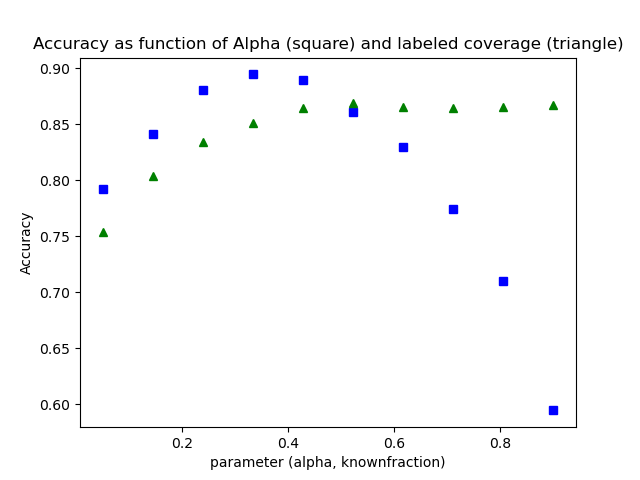
\includegraphics[width=\textwidth]{figures/alpha_fraq_graph.png}
%\caption{The accuracy as function of the resart parameter alpha,
%with fixed label coverage of 0.5, and of the label coverage with
%fixed alpha=0.2}
%\label{fig:alpha_fracs}
%\end{framed}
%\end{figure}

%\subsection{Discussion}
%If we look at figure \ref{fig:largest_connected_comp} which shows the connected
%component that we worked with, the red and blue are pretty nicely clustered. The
%greens and specially the yellows are sort of spread all over the network and
%not nicely clustered. I don't know if this is a good example of a real world
%scenario.
%
%When we look at figure \ref{fig:my_prediction} it seems that most of the
%incorrect predictions are on nodes that seem 'peripheral' and  are not well
%connected to known nodes. Another source of mistakes seems to bee green nodes
%that are too close to the red cluster.
%
%Method 2 shows somewhat higher accuracy over the other methods but on the flip
%side it is an $O(n^2)$ method when optimized methods are used whereas methods
%3,4,5 are $O(n)$.







%tests
%\section{Tests}
%Here is a lemma with a reference
%\begin{lemma}
%\label{lemma:foo}
%This is Lemma Foo
%\end{lemma}
%
%The proof for lemma \ref{lemma:foo} is in the appendix.







%%%appendices
\appendix
%section
\newpage \section{Appendix: Linear algebra primer}

\subsection*{}

\subsection*{}

\begin{mydef}
\label{Ax:def:transition} A \textbf{Transition Matrix } (we call
it a \textbf{Transition} in short), which is sometimes also called a
\textbf{stochastic matrix}, is a real valued non negative square
($n \times n$) matrix $A$ such that each of its columns sums up to one: $$A
\geq 0,\ \forall j \sum_i A_{i,j} = 1$$ $A$ acts from the left as a
linear mapping: $A:v \to A \cdot v$. In this paper we use left
multiplication convention ($Av$). There are many other publications
that deal with random walk and Markov processes, where right
multiplication is used ($v \cdot A$), and accordingly the rows are
normalized rather than the columns.

A transition is \textbf{positive}, designated by $A > 0$ if all its entries are positive.

A transition is \textbf{primitive} if for some $k>$ $A^k$ is positive. The same
property is called \textbf{regular} in some other sources.

A transition is \textbf{irreducible} if for every entry $A_{i,j}$ there is some $k$ such
that $A^k_{i,j} > 0$.

It can be shown that 
A matrix $A$ is 
irreducible by and only if it is NOT
similar by permutations matrices to a block upper triangular matrix
which means 
$
\nexists P : 
A =
P
\begin{pmatrix}
B & C \\
0 & D
\end{pmatrix}
P^{-1}
$

where $P$ is a permutation matrix and $B, C$ are square matrices of size greater than $0$.
\end{mydef}

\begin{mydef}
\label{Ax:def:state}
A \textbf{State} is a non-negative vector $v \in R^n$ s.t $\sum_i v_i = 1$.
\end{mydef}

\begin{remark}
\label{Ax:remark:state}
If $v$ is a
state and $A$ is a transition as defined in
\ref{Ax:def:transition}, then
  $Av$ is also a state because: 
$$\sum_i(Av)_i = \sum_j v_j(\sum_k A_{j,k}) = \sum_j v_j \cdot 1 = 1$$
Also its easy to confirm by multiplying with $e_i$, that if $Av$ is a state
for every state $v$ 
each column $A e_i$ must sum to $1$.
Therefore this is an equivalent definition for a transition.

If $A$ is a transition and $x,y$ are two states such that
$x \leq Ay$ then $x=y$.
\end{remark}

\begin{mydef}
\label{Ax:def:abs}
%changed C to R per Martin's request but it holds for C
Given $A \in \R^{n \times n}$ We let $|A| \in \R^{n \times n}$ be the resulting
matrix from applying $|\cdot|$ element wise. Given a vector $v \in \C^n$ we let
$|v| \in \R^n$ the corresponding non-negative vector.

We also let $A \gt 0, v \gt 0$ mean that it holds coordinate wise. 
\end{mydef}

Here is a very useful lemma for non-negative matrices which we will need later:
\begin{lemma}
\label{Ax:lem:eqal_by_vector}
Let $0 \leq A \leq B \in \R^{n \times n}$ 
and let $0 \lt v \in \R^n$.
If $Av = Bv$ then $A = B$.
\begin{proof}
Trivial.
\end{proof}
\end{lemma}

\begin{remark}
\label{Ax:remark:abs}
If $u \in \C^n$ is on the unit circle and $T$ a transition then
$|u|$ is a state, meaning $\||u|\|_1=1$, so $T|u|$ is also a state 
so $\|T|u|\|_1=1$.

We have (component-wise) $|Tu| \leq T|u|$. If $T>0$ and $u$ has negative or
non-real entries, then this inequality must be strict and
then $\|Tu\|_1 \lt \|T|u|\|_1 = 1$.
\end{remark}

\begin{lemma}
\label{Ax:lem:exist1}
If $T$ is a transition, then
there is a state $u$ such that $Tu = u$.
\begin{proof}
Because the columns of $A$ all sum to $1$, the columns of $A-I$ all sum to $0$.
Therefore $(1,1, \dots, 1)$ is an (left) eigenvector of the rows with eigenvalue $1$.
Therefore there is also some real (right) column eigenvector with eigenvalue $1$. 
(Also it follows from the Brouer fixed point theorem because $T$ maps the $l_1$
sphere to itself).

Let $u \in R^n$ be such vector: $Au=u$. Let $u = u^+ + u^-$ such that $u^- =
\min(u_i,0)$ and the other one defined similarly for the non-negative components.

Because $A$ is non-negative $A(u^+) \geq (Au)^+ \geq 0$,
and $A(u^-) \leq (Au)^- \leq 0$.

From $A$ being
non-negative and $(Au)^+ + (Au)^- = Au = u = u^+ + u^-$
And also $(A u)^+ = (u)^+$, so we must have $Au^+ \geq (Au)^+ = u^+$ 
(component wise). But if we had a strict inequality we would get:
$\|A(u^+/\|u^+\|_1)\|_1 > 1$ which is a contradiction to $A$ being a transition
matrix.

Then $A u^+ = u^+, A u^- = u^-$ and one of them must be non-zero. It follows
that $A$ has a non-negative eigenvector with eigenvalue $1$ (one of $u^+, -u^-$
which is non-zero). If we $l_1$-normalize that eigenvector it becomes a state.
\end{proof}
\end{lemma}


\begin{lemma}
\label{Ax:lem:uniq1}
If a transition $A \gt 0$ (or primitive)
, then it has exactly
one eigenvector $v$ with eigenvalue $1$ and in addition $v$ can be
chosen to be strictly positive.
Furthermore, for any other eigenvalue
$\lambda$ it holds that $|\lambda| \lt 1$.

If $A$ is just irreducible then then again $v>0$ and is unique but there may be
additional eigenvalues on the unit circle.

\begin{proof}
Let $A \gt 0$ be a transition. We already know that there exists at least one such eigenvector.
Let $u,v$ s.t $Au=u, Av=v$. 
We can assume these are real vectors because $A$ has only real entries.
Therefore we can choose $u,v$
to be states as we have already proven above.

Then let $w=u-v$. So $Aw = A(u-v) = u-v = w$. 
And $\sum_i w_i = 1 - 1 = 0$ by choice of $u,v$.

Like before $Aw^+ = w^+, Aw^- = w^-$
and because $w \neq 0$ but sums up to $0$, both $w^+, -w^- > 0$.
Because $w^-$ is non zero exactly on entries where $w^+$ is zero and vice versa, 
each of them must have at least one $0$ entry (and one none zero). But because
$A$ is strictly positive and $w^+$ is non-negative, $Aw^+$ must have ONLY
positive entries, contradicting $Aw^+ = w^+$. It follows then that $u-v=0$ is
the only possibility, hence the eigenvector with $1$ as eigenvalue is unique.

Suppose there is $Aw = \lambda w$ where $| \lambda|=1$. Choose $w$ so it is
$l_1$-normalized. Then $|w| = |Aw| \leq A \cdot |w|$ If $w$ has any negative or
complex coordinantes, then $|Aw| \lt A|w|$ and therefore 
$1 = \| |Aw| \|_1 \lt \|A|w|\|_1 =1$, a contradiction. Therefore there cannot be
any other eigenvalues on the unit circle.

Extending this for primitive matrix is easy because for some sufficiently big
$k$ $A^k \gt 0$. 

To prove the uniqueness of the $1$-eigenvector for the irreducible case, we have
$(\forall k \in \N) A^kw^+ = w^+$ and from that with some more work left undone
it follows that $w^+ > 0$ or
$w^+ = 0$.
\qedsymbol

\end{proof}
\end{lemma}

\begin{remark}
\label{Ax:remark:rhoisone}
The lemmas and theorems in this section are phrased in term of transitions. They
hold true in the more general case of positive/non-negative
linear transformations and one just replaces $1$ with the \textbf{spectral
radius} $ \rho = \rho(A)$.

In general a non-negative linear transformation has a \textbf{spectral radius}
$\rho = \rho(A)$ which is the absolute value of its greatest eigenvalue. In the case of
positive maps there is a unique single eigenvector with $\rho$ as the unique
greatest eigenvalue and so forth \dots. When we deal with a transition map,
lemma \ref{Ax:lem:uniq1} guaranties 
it has a spectral value of $\rho(A) = 1$.
\end{remark}

\begin{thm}
\label{Ax:thm:transition_ev}
Let $T$ be a positive (or primitive) transition. Then 

1. $1$ is the greatest eigenvalue
of $T$ and it has one unique eigenvector which is also positive,
so there exists a unique stationary state.

2. All the other eigenvalues have absolute value strictly less than $1$.

3. For every state $u$, $T^ku$ converges to the stationary state $\pi$.
In particular the columns of $T^k$ converge to $\pi$.

\begin{proof}
1 and 2. We already know.

3. There is a Jordan decomposition $T = PJP^{-1}$, such that $J$ is a Jordan
matrix, $J_{1,1} = 1$ and the rest of the main diagonal $|J_{i,i}| <1$.
So now the convergence is clear $J^k \to (e_1 | 0 \dots | 0)$.
For the matrix $P$ it must hold that $P = (P_1| \dots| P_n)$ and $P_1$ is the column 
eigenvector of $T$ corresponding to $1$ which we are free to $l_1$ normalize 
and the first row of $P^{-1}$ is the
left eigenvector corresponding to $1$ and so force \dots.

Some more work or literature check should confirm that $T^k \to (v|v\dots|v) = V$.
Then one can verify $Vu = v$ for any state $u$.
\end{proof}
\end{thm}

\begin{thm}
\label{Ax:thm:transition_irr_ev}
Let $T$ be an irreducible positive (or primitive) transition. 
Then:

1. Then $1$ is the greatest eigenvalue
of $T$ and it has one unique eigenvector which is also positive,
so there exists a unique stationary state.

2. If there are other other eigenvalues on the unit circle then their algebaic
multiplicity is equal their geometric multiplicity.

3. For every state $u$, the \textbf{Cesaro sums} 
$\frac{1}{n}\sum_{k=1}^n T^ku$ converge to the stationary state $\pi$.

\begin{proof}
1 We already know.

2. There is a Jordan decomposition $T = PJP^{-1}$. such that $J$ is a Jordan
matrix, $j_{1,1} = 1$ and the rest of the main diagonal $|J_{i,i}| \leq 1$.

If we had a Jordan block of size greater than $1$ for an eigenvalue $\lambda$,
Then on the superdiagonal of $J^k$ we would have $k \lambda$. If $|\lambda| =1$
then $J^k$ and hence $T^k$ would be unbounded, but that is impossible since
$T^k$ is a transition. If follows that all eigenvalues on the unit circle must
be semi simple (alebgaic multiplicity equals geometric).

3. For the convergence, it follows from calculations on the Jordan blocks, which
I omit. See \textcite{meyer2000matrix} or \textcite{serre2010matrices}
for rigorous proof.
\end{proof}
\end{thm}

What differs irreducible non-primitive matrices from primitive is
that they are periodical on their eigenvectors with complex eigenvalues
on the unit cycle. There is, in fact a wonderful theorem from Wielandt which
characterizes these Matrices:

\begin{thm}[Wielandt (1950)]
\label{Ax:thm:wielandt}
Let $A,B \in \C^{n \times n}$ such that $A \geq 0$ is irreducible and $|B| \leq
A$ (component-wise). Then $\rho(B) \leq \rho(A)$.
If $\rho(B)=\rho(A)$ then $|B|=A$, $B$ has an eigenvalue of the form $\mu =
\rho(A)e^{i \phi}$ and:

\begin{equation}
\begin{aligned}
\label{Ax:eq:wielandt1}
B &= 
e^{i \phi}DAD^{-1} \\ 
\text{where } D \text{ has the form:}\\
D &= 
\begin{pmatrix}
e^{\theta_1} & & & \\
& e^{\theta_2} & & \\
& & \ddots & \\
& & & e^{\theta_2}
\end{pmatrix}
\end{aligned}
\end{equation}

And conversely any $B$ of the form \ref{Ax:eq:wielandt1}
has $\rho(B) = \rho(A)$, $|B|=A$ and $\mu$ is an eigenvalue of $B$ which
corresponds to the eigenvalue $\rho(A)=|\mu|$ the greatest eigenvalue of $A$.

\begin{proof}
To see a rigorous proof I suggest \textcite{meyer2000matrix}.

The keys for proving this theorem are:
First WLG assume $A$ is a transition. This is possible because we may replace
$A$ with $AW^{-1}$, and $B$ with
$BW^{-1}$, where $W$ is the diagonal matrix that has the column-sums of $A$.
Since $A$ is irreducible it cannot have a column or a row that is all $0$
so this diagonal is positive $W$ is indeed invertible and later we can cancel out the
$W$'s and return to the general case.

Let $v$ be the $\mu$-eigenvector $Bv = \mu v, \|\mu|=1$ and choose it so that 
$\|v\|_1=1$.

Then 
\begin{equation}
|v| = |\mu v| = |B v| \leq |B| |v|
\leq A |v|
\end{equation}

Since $A$ is a transition by remark \ref{Ax:remark:state} $A|v|=|v|$. Since $A$ is
irreducible and $A|v| = |v|$ we must have by \ref{Ax:thm:transition_irr_ev} that
$|v| \gt 0$, and then by
lemma \ref{Ax:lem:eqal_by_vector} $A = |B|$ so that proves the first part.  

Now let $w = v / |v|$ (component-wise division) and let 
\[D = \text{diag}(w) = 
\begin{pmatrix}
e^{\theta_1} & & & \\
& e^{\theta_2} & & \\
& & \ddots & \\
& & & e^{\theta_2}
\end{pmatrix}
\]

Then $v = D|v|$, $|v|=D^{-1}v$ and we have:

\begin{equation}
\label{Ax:eq:wielandt1proof}
\begin{aligned}
A|v| &= |v| = D^{-1}v = \\
&= D^{-1} \mu^{-1} B v = \mu^{-1} D^{-1} BD|v|
\end{aligned}
\end{equation}

We know already that $|v| \gt 0$. If 
$C := \mu^{-1} D^{-1} BD$ contains any negative or complex entries, then
\ref{Ax:eq:wielandt1proof} cannot hold. It follows that
\[
A = C = \mu^{-1} D^{-1} BD 
\]

This proves the harder direction of the claim, the other direction is easy \qedsymbol.

\end{proof}
\end{thm}

The amazing consequence from \ref{Ax:thm:wielandt}:

\begin{thm}[Corollarly]
\label{Ax:thm:wielandt2}
If $A$ is irreducible transition with $h$ 
eigenvalues on the unit circle then its eigenvalues are exactly the $h$th unit roots
$\lambda_k = e^{2 \pi i k /h}, k = 0 \dots n-1$ and $A$ is similar to $\lambda
A$ by a diagonal matrix for any such eigenvalue.

\begin{proof}
Use theorem \ref{Ax:thm:wielandt} with $B=A$. If $|\lambda|=1$ is an eigenvalue
then $A = \lambda D A D^{-1}$. Since similarity doesn't change the eigenvalues,
$A$ and $\lambda A$ must have the same eigenvalues with the same multiplicity.
Since $1$ is a simple eigenvalue of $A$ and hence of $\lambda A$, and its
corresponding eigenvalue $\lambda$ is simple in $\lambda A$ and therefore in $A$
as well.

The matrices $\lambda_k A$, $k=0 \dots h$ are all similar, with $\lambda_0 = 1$
and $|\lambda_k| = 1, k=0 \dot h-1$ all simple eigenvalues. The only way for this to hold is if
$\{\lambda_k\}_0^{h-1}$ form a multiplicative group of order $h$ on the unit
circle, in other words, the eigenvalues are exactly all the $h$th unit roots. 
\end{proof}
\end{thm}

\begin{remark}
\label{Ax:remark:wielandt_cyclicity}
If $A$ is irreducible transition with exactly $h$ 
eigenvalues on the unit circle then $h$ is called the \textbf{period} of $A$.
$A \geq 0$ is primitive if and only if it is irreducible and aperiodic ($h=1$).

If $\omega = e^{2 \pi i /h}$ then \ref{Ax:thm:wielandt2} shows that $A = \omega D A
D^{-1}$. So if $\lambda$ is any eigenvalue not necessarily on the unit circle,
then $\omega \lambda$ is also an eigenvalue with the same multiplicity and
rotation with $\omega$ is an automorphism on the eigenvalues.

We may choose $D$ so that $D[1,1]=1$. If we reindex the dimension we can make
$D$ look like 
\[
D = [D_0 | \omega D_1 | \dots \omega^{h-1} D_{h-1}]
\] So Indexes corresponding to the same phase of the period appear sequentially.


Then use the identify $\forall k D^hA^{k} = A^k D^h$ and the fact that $A$ is
irreducible to show that $D^h = I$. Then use the identity $\omega DA = AD$ to
show that in the new indexing $A$ has the following periodical block structure
($0$ on the main diagonal):

\[
A = 
\begin{pmatrix}
0 & M_1 & 0 & \dots & 0 \\
0 & 0 & M_2 & 0 \dots & 0 \\
 &  & \ddots & \ddots & &  \\
0 & \dots & 0 & 0 & M_{h-1} \\
M_h & 0 & \dots & 0 & 0 
\end{pmatrix}
\]
\end{remark}


Now we will just present the Perron-Frobenius theorems. The main parts that are
important to our work have appeared in the previous theorems.

\begin{thm}[Perron-Frobenius \cite{meyer2000matrix}]
\label{Ax:thm:perron1}


Let $0 \lt A \in \R^{n \times n}$ with spectral radius $\rho := \rho(A)$, then the following are all true:
\begin{itemize}
\item{} $\rho \gt 0$
\item{} $\rho$ is a simple root of the characteristic polynomial of $A$,
in other words its algebraic multiplicity is $1$.
\item{} $(\exists v > 0) Av=\rho v$
\item{} If $Au = \lambda u$ and $\|u\|= \rho$ then $\lambda = \rho$
namely, $\rho$ is the unique eigenvalue on the spectral circle.
\item{(Collatz-Wielandt Formula)} $\rho = \max_{x \in \Gamma} \min_{i : x_i \neq 0} [Ax]_i / x_i$
with $\Gamma = \{x | x \geq 0, x \neq 0\}$
\end{itemize}
\end{thm}

\begin{thm}[Perron-Frobenius for irreducible matrices \autocite{meyer2000matrix}]
\label{Ax:thm:perron2}

Let $0 \leq A \in \R^{n \times n}$ be irreducible with spectral radius $\rho := \rho(A)$,
then the following are all true:
\begin{itemize}
\item{} $\rho \gt 0$
\item{} $\rho$ is a simple root of the characteristic polynomial of $A$,
in other words its algebraic multiplicity is $1$.
\item{} $(\exists v > 0) Av=\rho v$
\item{} There are no additional non-negative unit eigenvectors of $A$ other than
$v$. 
\item{(Collatz-Wielandt Formula)} $\rho = \max_{x \in \Gamma} \min_{i : x_i \neq 0} [Ax]_i / x_i$
with $\Gamma = \{x | x \geq 0, x \neq 0\}$
\end{itemize}
\end{thm}




%section
\newpage \section{Appendix: More on matrices, graphs and stochastics}
\subsection*{}

\subsection*{}

A directed non-weighted graph $G$ can be uniquely represented by its
\textbf{adjacency matrix},
$A_{i,j} := 1$ if and only if there is a directed edge from $j$ to $i$ (if we
want to use it for transitioning on columns as done above). It's possible to
assign different edge weights rather than only $1$ and $0$. If the graph is
undirected each edge would be counted in both directions and the matrix is
symmetric.
Relabeling the vertices of a graph yields an adjacency matrix that is similar by
permutations ($PAP^{-1}$, where $P$ is a permutation matrix) and vice versa.

To turn $A$ into a transition, normalize each column by dividing it with
its out going rank, so let $D_{i,i} = \text{out~rank}(i)$, $T:=AD^{-1}$ is the
transition matrix of this graph (because right-multiplying by $D$ normalizes each
column by its rank).
If the graph was stochastic to begin with then the adjacency matrix as we
defined it is already column-normalized.

\begin{mydef}
\label{Ax:def:stronglyconnected}
A graph is $G$ \textbf{strongly connected} if there is a directed path form any edge
to any edge. Equivalently $G$ is strongly connected if and only if its adjacency matrix is irreducible.

We say that the \textbf{Period of a vertex} $v \in V(G)$ is the greatest common
divisor of all closed paths on $v$. If the periods of all vertices are equal
(spoiler: in the case that $G$ is strongly connected they are), we call it the
\textbf{Period of the graph} $G$.
\end{mydef}

\begin{remark}
\label{Ax:remark:periods}
If $G$ is strongly connected then the periods of all vertices are indeed equal
and its easy to prove. The corresponding adjacency matrix $A$ is irreducible so
it too has a period $h$ as defined in \ref{Ax:remark:wielandt_cyclicity} and it is
equal to the graph period (can be shown using \ref{Ax:thm:wielandt2} and
\ref{Ax:remark:wielandt_cyclicity}).

So if the graph $G$ is strongly connected and has period $1$
then the adjacency matrix is \textbf{aperiodic} and hence primitive, and vice versa. 
\end{remark}

From all the above we have seen that a Markov process can be represented in two
equivalent ways \textemdash as a transition matrix  and as the 
corresponding weighted directed graph.

If the graph $G$ is strongly connected and aperiodic, its corresponding
adjacency matrix is primitive. We know from \ref{Ax:thm:perron1} that there is a
unique stationary distribution $p$ and that the Markov process converges to $p$ no
matter from which distribution it starts. We may calculate $p$ using the
\textbf{power
method} which is efficient because it can be done in a matrix-free method. 
%We don't need to know the matrix itself just the dot product of it with a state
%vector.

If the graph $G$ is strongly connected, then \ref{Ax:thm:perron2} assures us the
existence and uniqueness of a stationary distribution $p$. But if $G$ is not
aperiodic, the corresponding adjacency matrix is not primitive. We cannot use
the efficient power method to calculate $p$. Also the process itself doesn't
stabilize on $p$. It is periodic and cycles between the $h$ eigenvectors on
the unit circle (see theorem \ref{Ax:thm:wielandt2}). 

We are therefore interested to find how to convert an \text{imprimitive}
matrix (= irreducible but not primitive)
to a primitive matrix or equivalently to turn a strongly connected but periodic graph
into an aperiodic graph.

\begin{lemma}\cite{meyer2000matrix}
\label{Ax:lem:1plusA}
Let $A \geq 0$ be irreducible. Then $(A + I)^{n-1} \gt 0$, and therefore $A+I$
is primitive.
\begin{proof}
Notice that the $I$ represents self loops and it absorbs all the lower powers so
if $(A^k)_{i,j} \gt 0$ for some $k \lt n$ then so is $(A+I)^{n-11}$.
Let $G := G_A$ be the corresponding graph to $A$. Then $G$ is strongly
connected. For every $i \neq j$ there is a directed \textbf{shortest path}
$\sigma$ in $G$ from $i$ to $j$. Its length must be $|\sigma| \lt n$. Otherwise
$\sigma$ would have to contain a cycle and not be of minimal length.
This shows that we have for every $i \neq j$ some $k$ sucht that $A^k_{i,j} \gt
0$ and therefore $(A+I)^{n-1} \gt 0$.
\end{proof}
\end{lemma}

The properties of irreducibility, primitiveness and positivity only depend on the
sign ($-,0,+$) of the entries and not on their size. So we use the following definition to
test matrices for these properties:

\begin{mydef}
Let $A \in \R^{n \times n}$, then its \text{binary form} is the matrix
$\beta(A) := \text{sgn}(A)$ where $\text{sgn}$ is applied element-wise.
\end{mydef}

The following trivial lemmas would help as to construct primitive transitions:

\begin{lemma}
\label{Ax:lemma:SplusT}
$A$ is positive/primitive/irreducibly if
and only if $\beta(A)$ is.

Let $0 \leq \beta(A) \leq \beta(B)$.
Then If $A$ is positive/primitive/irreducibly so is $B$.

Let $0 \lt \alpha \lt 1$. If $T,S$ are transitions the so is $W=(1-\alpha)T +
\alpha S$.
If one of $S,T$ is positive/primitive/irreducible so is $W$
\end{lemma}

Let $G$ be any weighted graph and $A$ its adjacency transition matrix. Some vertices may
be unreachable from other vertices and there might not exist a single and
unique stationary distribution.
A random walk on this graph is generally
dependent on the initial starting distribution $p_0$ and has the
form $p_{k+1} = Ap_k = \dots = A^k p_0$, where $p_k$ is the
distribution after $k$ steps.

However if we allow the possibility of 'random restart' from any state, this
graph becomes totally connected it is guarantied to have a unique stationary
distribution to which any random walk converges regardless of the initial state.

When we talk about \textbf{random walk with restart (RWR)} we set a restart
state $q$ and a restart parameter $\alpha \in [0,1]$. At each step, we
either restart over to the state $q$, with probability of
$alpha$, or continue to walk using the normalized adjacency matrix
$A$. The state sequence is therefore
\begin{equation}
\label{Ax:eq:RWR}
p_{k+1} = \alpha q + (1 -
\alpha) A \cdot p_k
\end{equation}

It turns out that this random walk with restart is actually a normal
random walk but with an modified adjacency matrix (and respectively, an
modified weighted directional graph). 

\begin{lemma}
\label{Ax:lemma:Qq}
Let $q$ be any state, let $\alpha \in [0,1]$ and let  
$ Q = (q|q|\dots|q)$ (The square matrix whose every column equals $q$).
Then $Q$ is a transition and for any state $p$ we have $Qp = Q$.

In addition if $T$ is any transition then $W = \alpha Q + (1-\alpha)
T$ is also a transition, And we can rewrite the RWR from
\ref{Ax:eq:RWR} as

$p_{k+1} = \alpha q + (1 - \alpha) Ap_k = 
[\alpha Q + (1 - \alpha) A] p_k = W p_k$

\begin{proof}
Trivial and uses \ref{Ax:lemma:SplusT}
\end{proof}
\end{lemma}

The matrix $W$ represents a graph $G'$ where each edge of the
original graph $G$ is rescaled by a factor $1 - \alpha$ (and if $G$ is
undirected we treat each undirected edge as $2$ directed edges in
$G'$. In addition from each vertex $v$ we add edges to every other
vertex and the weight of the additional edge is $\alpha q[u]$.

If we pick the restart state $q$ in a way that makes $W$ primitive,
then \ref{Ax:thm:perron1} assures us that the RWR will converge,
$\lim_{k \to \infty} p_k =\lim_{k \to \infty} W^k p_0 = p$, where
$p$ is the unique stationary distribution of $W$. This means in
particular that we can use the power method to find out the
distribution $p$ by sequentially calculating $p_1, p_2, \dots$ until
it sufficiently converges, and it will converge to $p$ from any
initial state $p_0$ which we choose. 

Also we can take the limit $p = \lim_{k \to \infty}p_k$ and rewrite
\ref{Ax:eq:RWR} as:
\begin{equation}
\label{Ax:eq:RWR2}
\begin{aligned}
p = Wp = \alpha q + (1 - \alpha) A \\
[I - (1 - \alpha)A] p = \alpha q
\end{aligned}
\end{equation}

We will see later that we can invert the matrix in the second
equation of \ref{Ax:eq:RWR2} and use a direct solution for $p$ instead of
the power method. The power method has the advantage that we can use
the matrix $A$ implictly, because we only need to know $A \cdot p_k$
to compute $p_{k+1}$. $A$ is usually a sparse matrix because each
vertex usually only has few neighbors and so we can use matrix free
methods efficiently to calculate $p$ but that is beyong the scope of
this thesis.

In the particular case of pageRank, we choose a uniform restart
state $q = \mathbf{\frac{1}{n}}$. The corresponding matrix $Q =
(q|\dots|q) \gt 0$ is strictly positive, and therefore 
$W = \alpha Q + (1 - \alpha)A > 0$ is positive and therefore
primitive.

The stationary distribution which corresponds to this uniform
restart state $q$ is called the \textbf{PageRnak} for $G$ with
restart parameter $\alpha$. It is used to order the vertices
according to their 'relevance' in the network.



The PageRank is the stationary distribution of the process when we use unbiased
restart\textemdash A restart is equally likely from any vertex.
But we want more. We want to find out what happens when we restart, for example,
always from one single vertex $u$. We think of the stationary distribution $p_u$ that 
results from such process as the heat (or flow) which propagates out of $u$.
If we take another vertex $v$ we think of $p_u[v]$ as a measure of how close $v$
is to $u$, or how much heat $u$ sends to $v$.
Note that this is not symmetric $p_v[u] \neq p_u[v]$ in general.

%(memo: add an illustration about asymmetry)

\begin{lemma}
\label{Ax:lem:AplusP}
Let $A \geq 0$ be irreducible. Let $B \geq 0$ have a positive row (or column),
then $A + B$ is primitive.
\begin{proof}
Suppose WLG that $B_1 > 0$ (first row). Then $\forall k \gt (B^k)_1 \gt 0$.
Fix $i,j$.
Since $A$ represents a strongly connected graph, there is a path from $i
\curvearrowright 1 \curvearrowright j$ of some length $k$. So $A^k_{i,j}>0$.
Then $\forall l \geq 0 (A + B)^{k+l} \gt 0$ because we can go along this path,
then self loop $l$ times in $1$ and keep going to $j$ on that path.

So we have shown that $(A+B)^k_{i,j}$ stays positive once it becomes positive
and it always turns positive at some point by irreducibility of $A$, so that
means $A+B$ is primitive.
\end{proof}
\end{lemma}

\begin{remark}
\label{Ax:rem:AplusP}
Lemma \ref{Ax:lem:AplusP} proves that we can propagate (namely do RWR) from any arbitrary restart
state $q$, including a single vertex and the combined transition matrix will be
primitive if the adjacency matrix $A$ is irreducible, or
equivalently, the corresponding graph $G$ is strongly connected.


Assume that $A$ is a normalized adjacency transition of a strongly
connected graph $G$.
Let $q$ be any state column vector, for example $e_1$ if we restart
from a single vertex, and let $Q = (q | q | \dots | q)$.
So $Q$ has a positive row and therefore $(1-\alpha)A + \alpha Q$ is a primitive
transition according to \ref{Ax:lem:AplusP}.

%Also worth noting that if $x \geq 0$ is any transition, then $Qx = q$.
\end{remark}

\begin{mydef}
\label{Ax:def:Transitionbiased}
Let $G$ be a graph with adjacency matrix $A$, and let $D$ be the
diagonal matrix of the out ranks of the vertices of $G$. Then we can
column normalize $A$ and create the transition $T = AD^{-1}$.
We define \textbf{the transition matrix with restart parameter}
$\alpha$ \textbf{and bias} $q$ as
\[
T_{\alpha, q} :=
(1 - \alpha)T + \alpha Q
\]
\end{mydef}

In general, 
the matrix $T_{\alpha,q}$ may have more than one unique stationary distribution $p$ 
(there is one for each strongly connected
component of its corresponding graph). But if we require that $G$ be
strongly connected (which means $A$ is irreducible),
then $T_{\alpha,q}$ is primitive by \ref{Ax:lem:AplusP}, and the
stationary distribution $p$ is unique.

\[
p = Ip
= [(1 - \alpha)T + \alpha Q]p =  (1 - \alpha)Tp + q 
\]

We can rearrange it now

\begin{equation}
\label{Ax:eq:uninvertedstationary}
(I - (1 - \alpha)T)p = \alpha q
\end{equation}

We want to invert the matrix in \ref{Ax:eq:uninvertedstationary} and use the
following lemma to justify it (The proof is easy. See for example
\textcite{serre2010matrices}):

\begin{lemma}
\label{Ax:lem:invertible}
Let $X$ be a contracting matrix, Then $(I-X)$ is invertible and the power sum of
$X$ converges to it:
\[
(I - X)^{-1} = \sum_{k=0}^{\infty} X^k
\]
\end{lemma}

So now we may apply lemma \ref{Ax:lem:invertible} on equation
\ref{Ax:eq:uninvertedstationary} because $(1-\alpha)A$ is contracting, and we have:

\begin{equation}
\label{Ax:eq:diffkernel}
p = \alpha [I - (1 - \alpha)T]^{-1} q := K q = 
\alpha \sum_{k=0}^{\infty} (1 - \alpha)^k T^k
\end{equation}

$K$ is called \textbf{diffusion matrix}~\cite{leiserson2015pan} of $T$ (or of the graph $G$) with parameter $\alpha$
It turns out that $K$ itself is a transition because it maps the
arbitrary transition $q$ to the transition $p$. In addition, $K \gt 0$ because
of \ref{Ax:eq:diffkernel} and since $T$ is irreducible.

What about the eigenvectors and eigenvalues of $K$?
If a matrix $A$ is invertible then $Av = \lambda v \iff A^{-1}v = \lambda^{-1}$.
For any matrix $Av = \lambda v \iff (I + A)v = (1+\lambda)v$.

It turns out then that $T$ and $K$ have the same eigenvectors and if $Tv=\lambda
v$ then $K v = \alpha [1 - (1 - \alpha) \lambda]^{-1} v$. And in particular if it
turns out that if all the eigenvalues are real (spoiler- they are), then they have
the same linear order as eigenvalues of $K$ or $T$ for the same eigenvector.
In particular we see that the choice of $\alpha$, the restart parameter, NEITHER 
changes the eigenvectors NOR does it change the order of the eigenvalues.

To sum up the important facts that we would need later:

\begin{thm}
\label{Ax:thm:AKTcharacteristics}
Let $G$ be strongly connected undirected graph. Let $A$ be its adjacency matrix
and $D$ the diagonal matrix which has the ranks of the vertices on its diagonal.
Let $T = A D^{-1}$, let $0 \lt \alpha \lt 1$ and 
$K = \alpha [I - (1 - \alpha)T]^{-1}$. Then the following are all true:

\begin{itemize}

\item{}
$A \geq 0$ is symmetric therefore its eigenvalues are all real.

\item{}
$T = AD^{-1} = D^{1/2}[D^{-1/2}AD^{-1/2}]D^{-1/2}$ is similar to $A$. Therefore
it has the same eigenvalues as $A$, which are all real:
$\lambda_1 \geq \dots \lambda_n$.

\item{}
There exists for all $0 \lt \alpha \lt 1$ the invertible matrix: 
$K := \alpha \sum_{k=0}^{\infty} (1 - \alpha)^k T^k = \alpha [I - (1 -
\alpha)T]^{-1}$.
$K \gt 0$ is a transition. It has the same eigenvectors as $T$ and their
corresponding eigenvalues are all real and they have the same order as the
corresponding eigenvalues for $T$ have.
\end{itemize}
\end{thm}

%The Equation looks something like this: Let $L = D - A$, the \textbf{Laplacian
%Matrix}. Let $\gamma \gt 0,$ and $0 \lt p_0 \in \R^n$ 



%section
\newpage \section{Appendix: Spectral clustering and other methods}
\subsection*{}

\textbf{Spectral Partitioning} 
\cite{von2007tutorial, naumov2016parallel, WikipediaGraphPartition, WikipediaSpectralClustering},
is a common technique for partitioning graphs. The idea is to construct a
Laplacian type matrix \cite{WikipediaLaplacianMatrix} for the graph
$G$,
analyze its eigenvalues and eigenvectors and construct a $2$-partition of $G$.
It is possible to create a hierarchical partitioning of $G$ by repeating the
process on each subdivision.

The problem of finding the best graph partition, also called the minimal cut
problem is NP-hard. Spectral partitioning methods are heuristics that
approximate the solution in 'real life' classes of networks.

\subsection*{}

\begin{mydef}
\label{def:Laplacian}
Let $G$ be a bidirectional graph with adjacency matrix $A$ and diagonal degree
matrix $D$.
Then the following matrices are its \textbf{graph Laplacian}, and its
\textbf{symmetric\textemdash
, row\textendash normalized\textemdash and column\textendash normalized\textemdash Laplacians}:  

\begin{equation}
\begin{aligned}
L & = D - A \\
L_s & = D^{-1/2}LD^{-1/2} = I - D^{-1/2}AD^{-1/2} \\
L_r & = D^{-1}L = I - D^{-1}A \\
L_c & = LD^{-1} = I - AD^{-1}
\end{aligned}
\end{equation}
\end{mydef}

Consider the connected graph $G$ and its adjacency matrix $A$. We create the transition
matrix by normalizing it: $T = AD^-1$, and finally we choose a restart parameter
$\alpha$ and create the diffusion matrix $K = \alpha[I - (1 -
\alpha) T]^{-1}$. Theorem
\ref{thm:AKTcharacteristics} assures us that $K$ and $T$ have the same
eigenvectors and the orders of their corresponding eigenvalues are the same. The
eigenvalues are all real and therefore the eigenvectors are real as well. And
the eigenvalues of $K$ are all non-negative.

The matrix $K^{-1} = \alpha^{-1} [I - (1- \alpha) T]$ is closely related to the
symmetric Laplacian $L_s$ and thecolumn-normalized Laplacian $L_c$. The added parameter $0 \lt \alpha \lt 1$
neither changes the eigenvectors, nor the order of the corresponding eigenvalues.

The smallest eigenvalue ,$0$ of $L$ and $L_s$
corresponds to the largest eigenvalue $1$ of and $T$ and its eigenvector is
(can be chosen as) all positive. 
Any other eigenvector of $L$ (which corresponds to an eigenvector of $T$) must
contain both positive and negative components due to \ref{thm:perron1}.

It's the eigenvector of the second smallest
eigenvalue $L$ or $L_s$ which is commonly used in 
They are commonly referred to as the \textbf{Fiedler} eigen-pair in the literature.
for spectral partitioning \cite{naumov2016parallel}. The simplest method is to
use the sign of the components of
eigenvector of the second smallest eigenvalue of $L$ or $L_s$.
This eigen-pair corresponds to the second largest eigenvalue of $T$

In \textcite{newman2006modularity} there is a particular type of spectral
partitioning which uses a matrix which the author called the modularity matrix.
It has the advantage over the Laplacian in that its greatest eigenvalue may be
positive or negative which is used to indicate or suggest the existence of
community structure in the graph. However the normalized Laplacians $L_r$ and
$L_c$ are more natural in the context of the random walk or propagation method
and recommended for example in \cite{von2007tutorial}.


\begin{figure}
\begin{framed}
\centering
\begin{subfigure}[b]{0.5\textwidth}
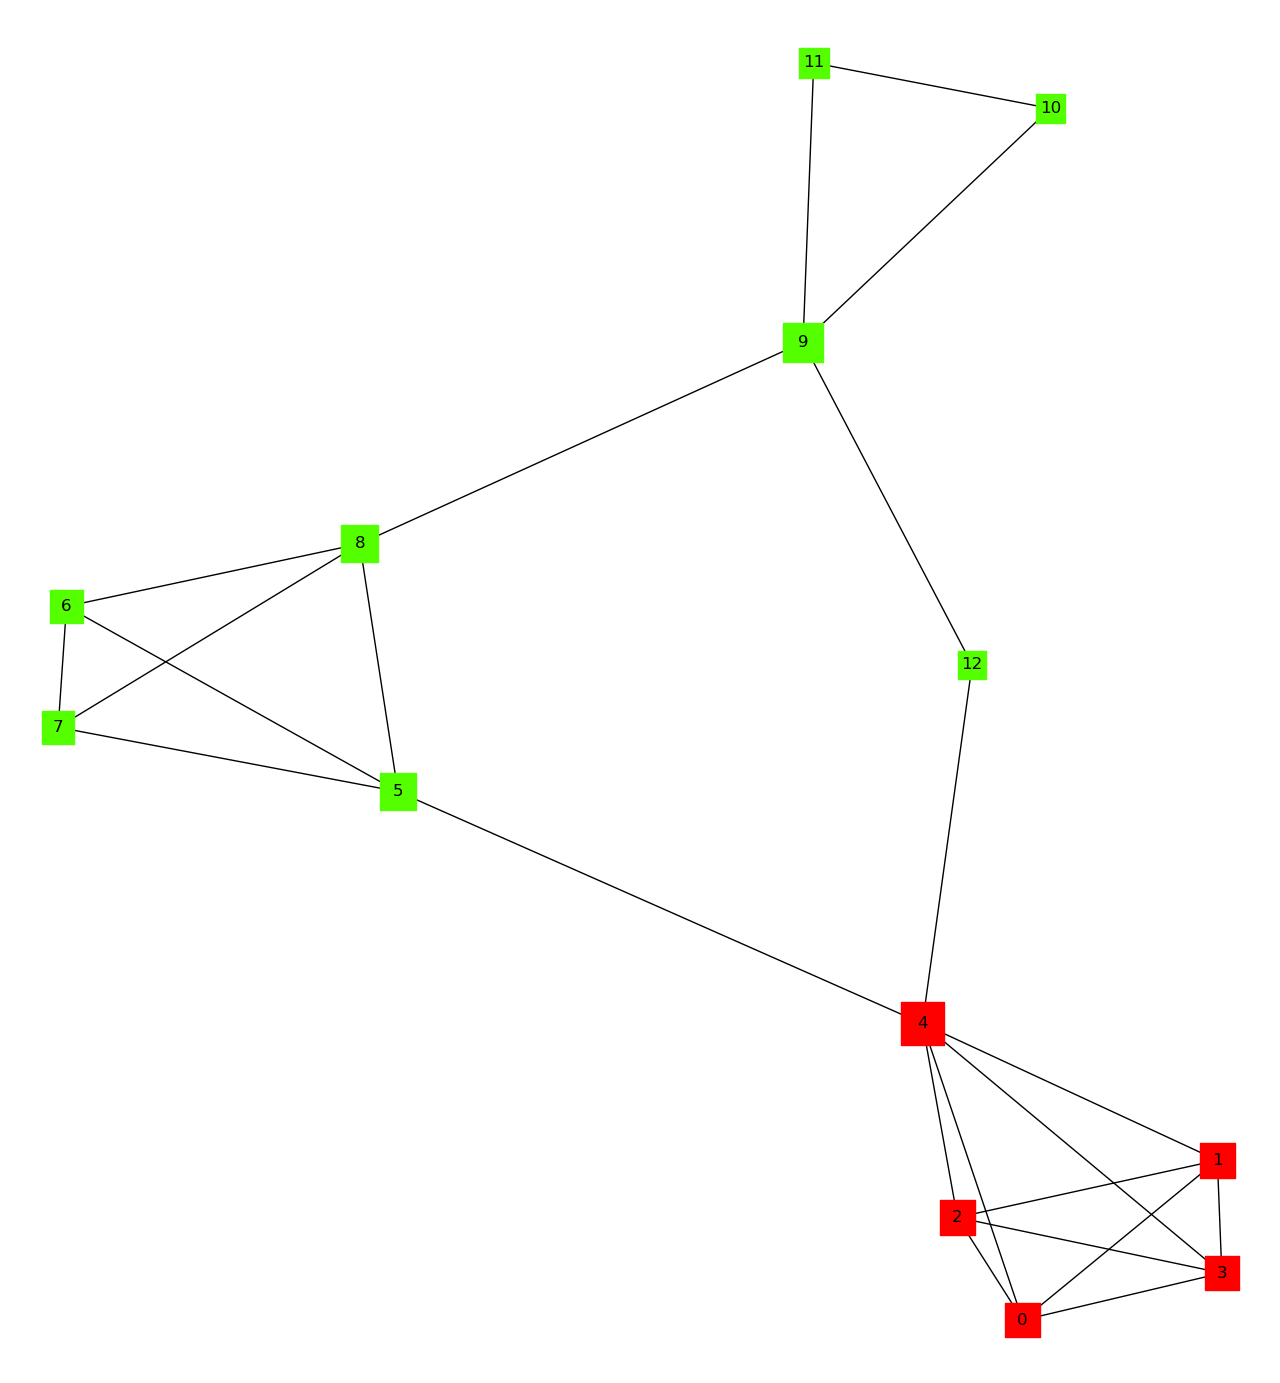
\includegraphics[width=\textwidth]{figures/example_spectralT2clustering.png}
\caption{A spectral clustering using the sign of the Fiedler eigenvector.}
\label{fig:toygraphspectralclustering}
\end{subfigure}
%add desired spacing between images, e. g. ~, \quad, \qquad, \hfill etc. 
%(or a blank line to force the subfigure onto a new line)
\begin{subfigure}[b]{0.5\textwidth}
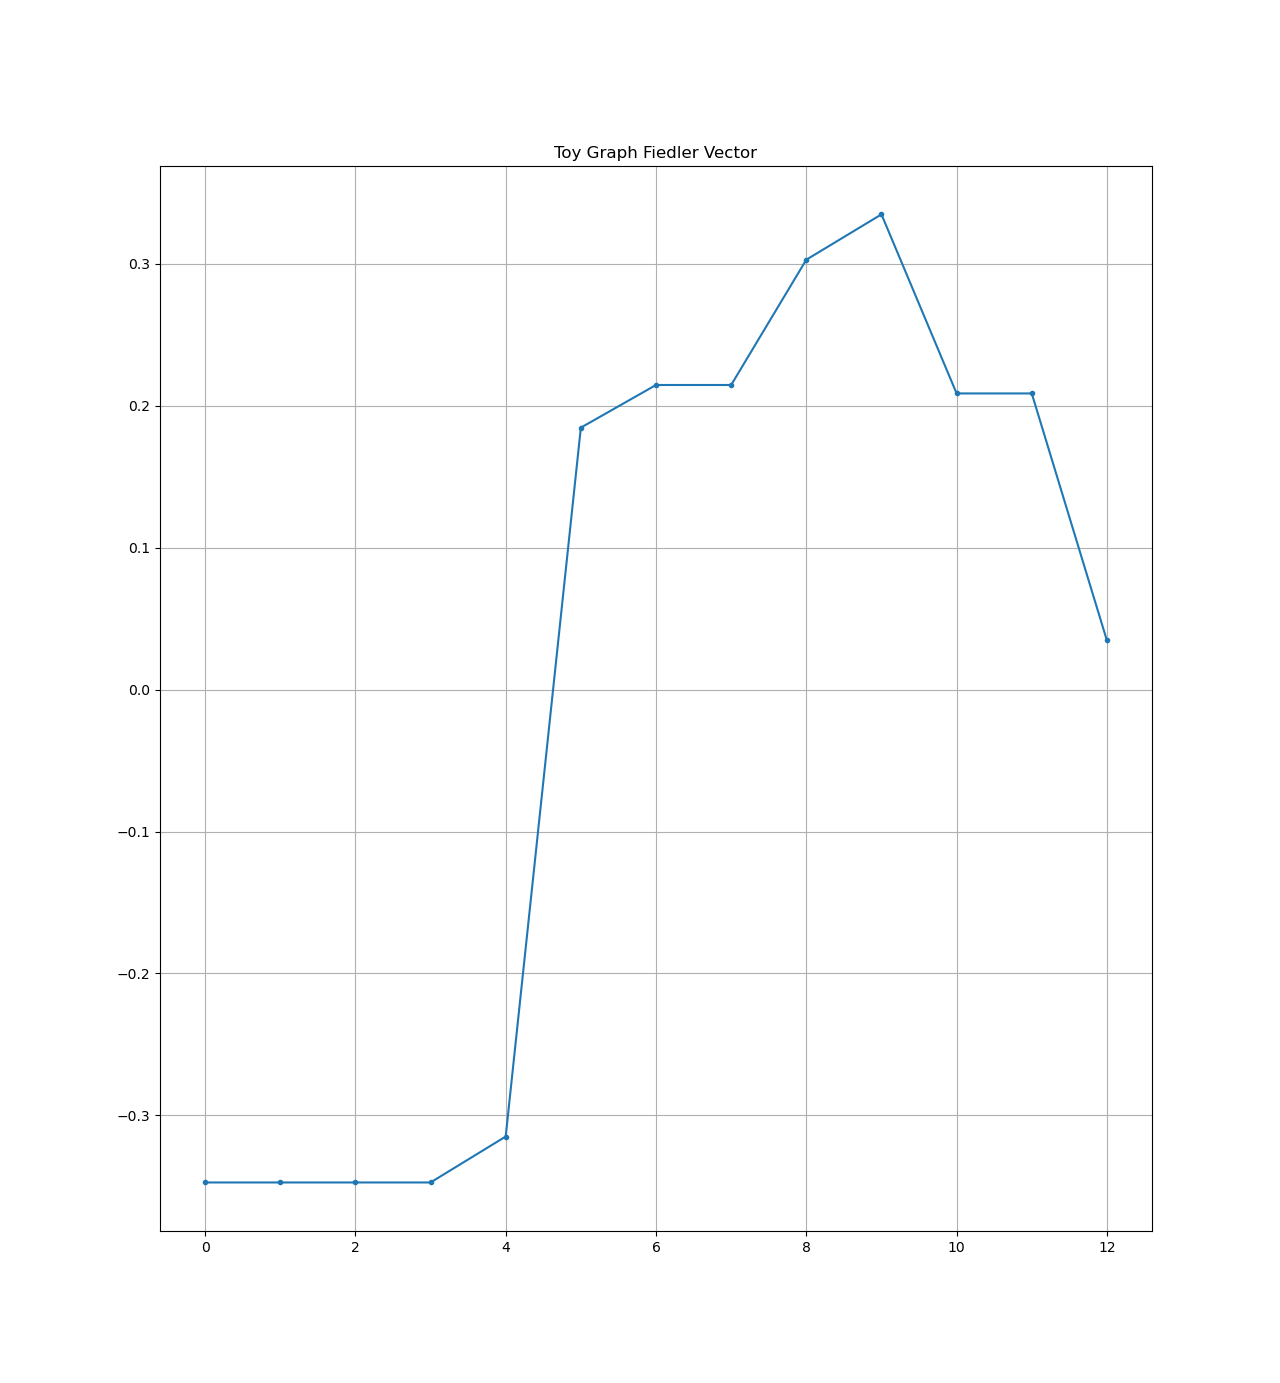
\includegraphics[width=\textwidth]{figures/Toygraph_Fiedler.png}
\caption{Plot of the Fiedler vector's components, showing a clear subdivision
between the positive and the negative components.}
\label{fig:toygraphfiedlerplot}
\end{subfigure}
%add desired spacing between images, e. g. ~, \quad, \qquad, \hfill etc. 
%(or a blank line to force the subfigure onto a new line)
\caption{}
%\label{fig:exampleCoolWarmClustering}
\end{framed}
\end{figure}

\begin{figure}
\begin{framed}
\centering
\begin{subfigure}[b]{0.5\textwidth}
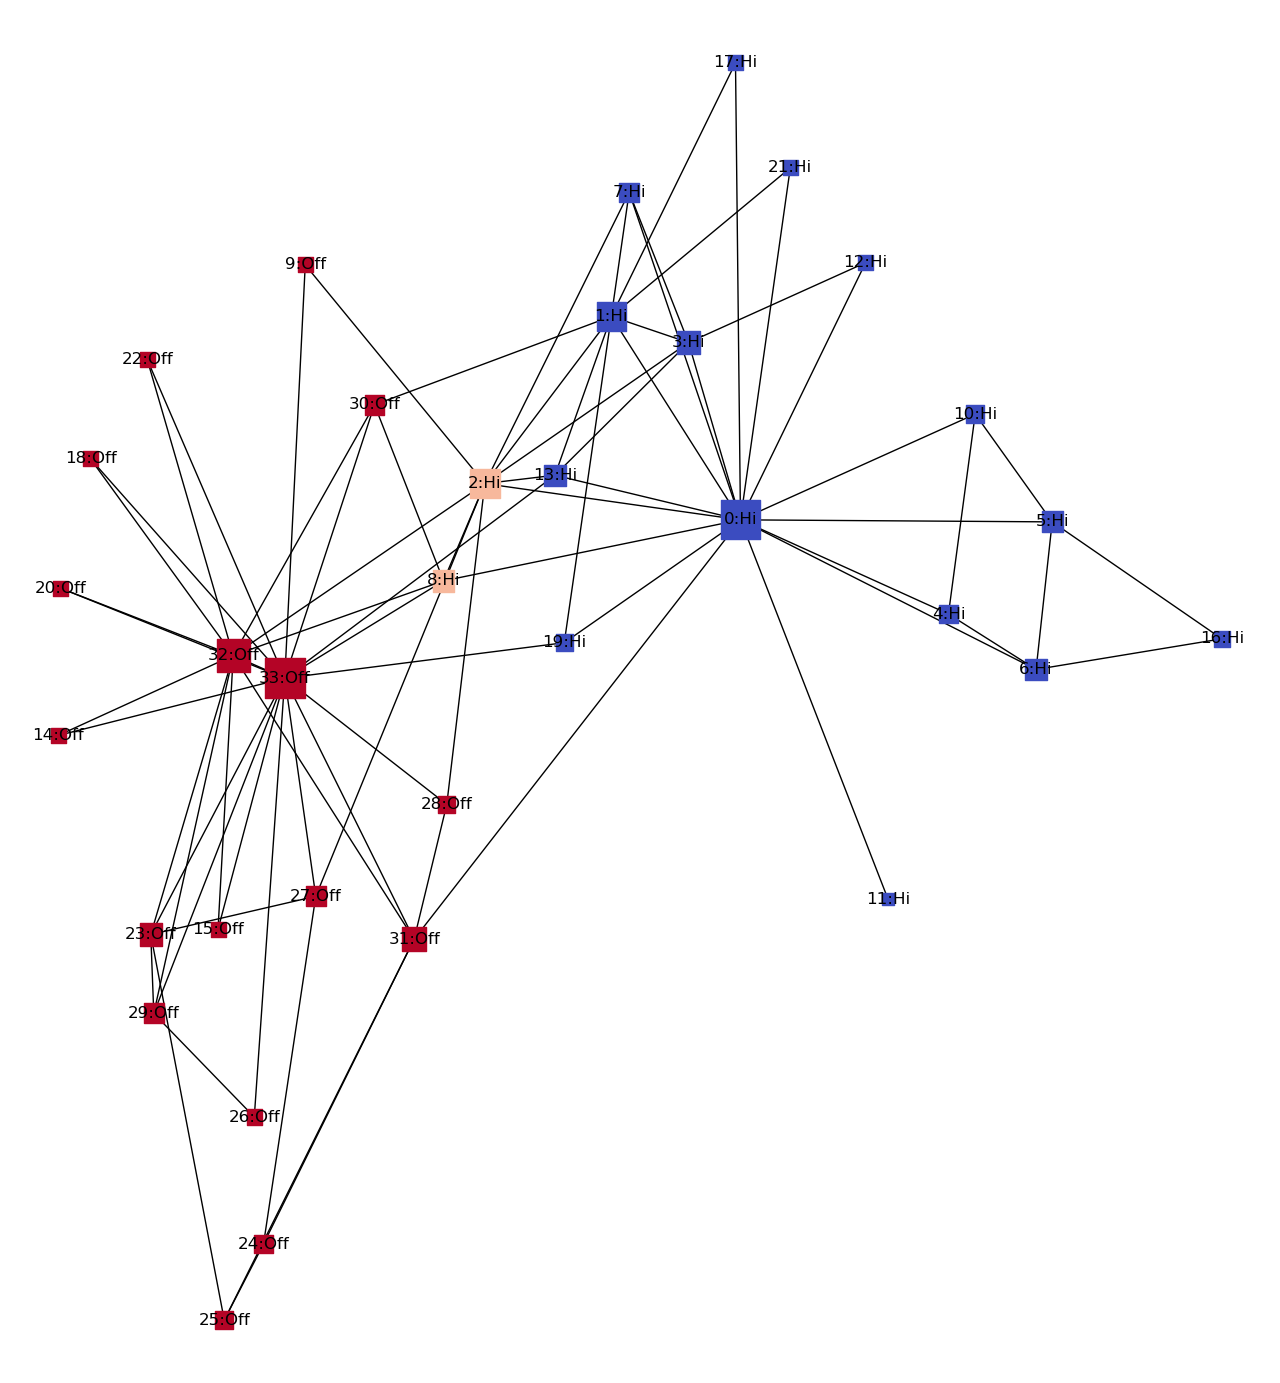
\includegraphics[width=\textwidth]{figures/Karate_spectralT2clustering.png}
\caption{Spectral clustering of the Karate Club network using the Fiedler
eigenvector signs. There are $2$ deviations from the actual partition, both are
borderline nodes which are harder to resolve. The $8$ node mistake is in common
with the naive algorithm of the previous section.}
\label{fig:karatespectral}
\end{subfigure}
%add desired spacing between images, e. g. ~, \quad, \qquad, \hfill etc. 
%(or a blank line to force the subfigure onto a new line)
\begin{subfigure}[b]{0.5\textwidth}
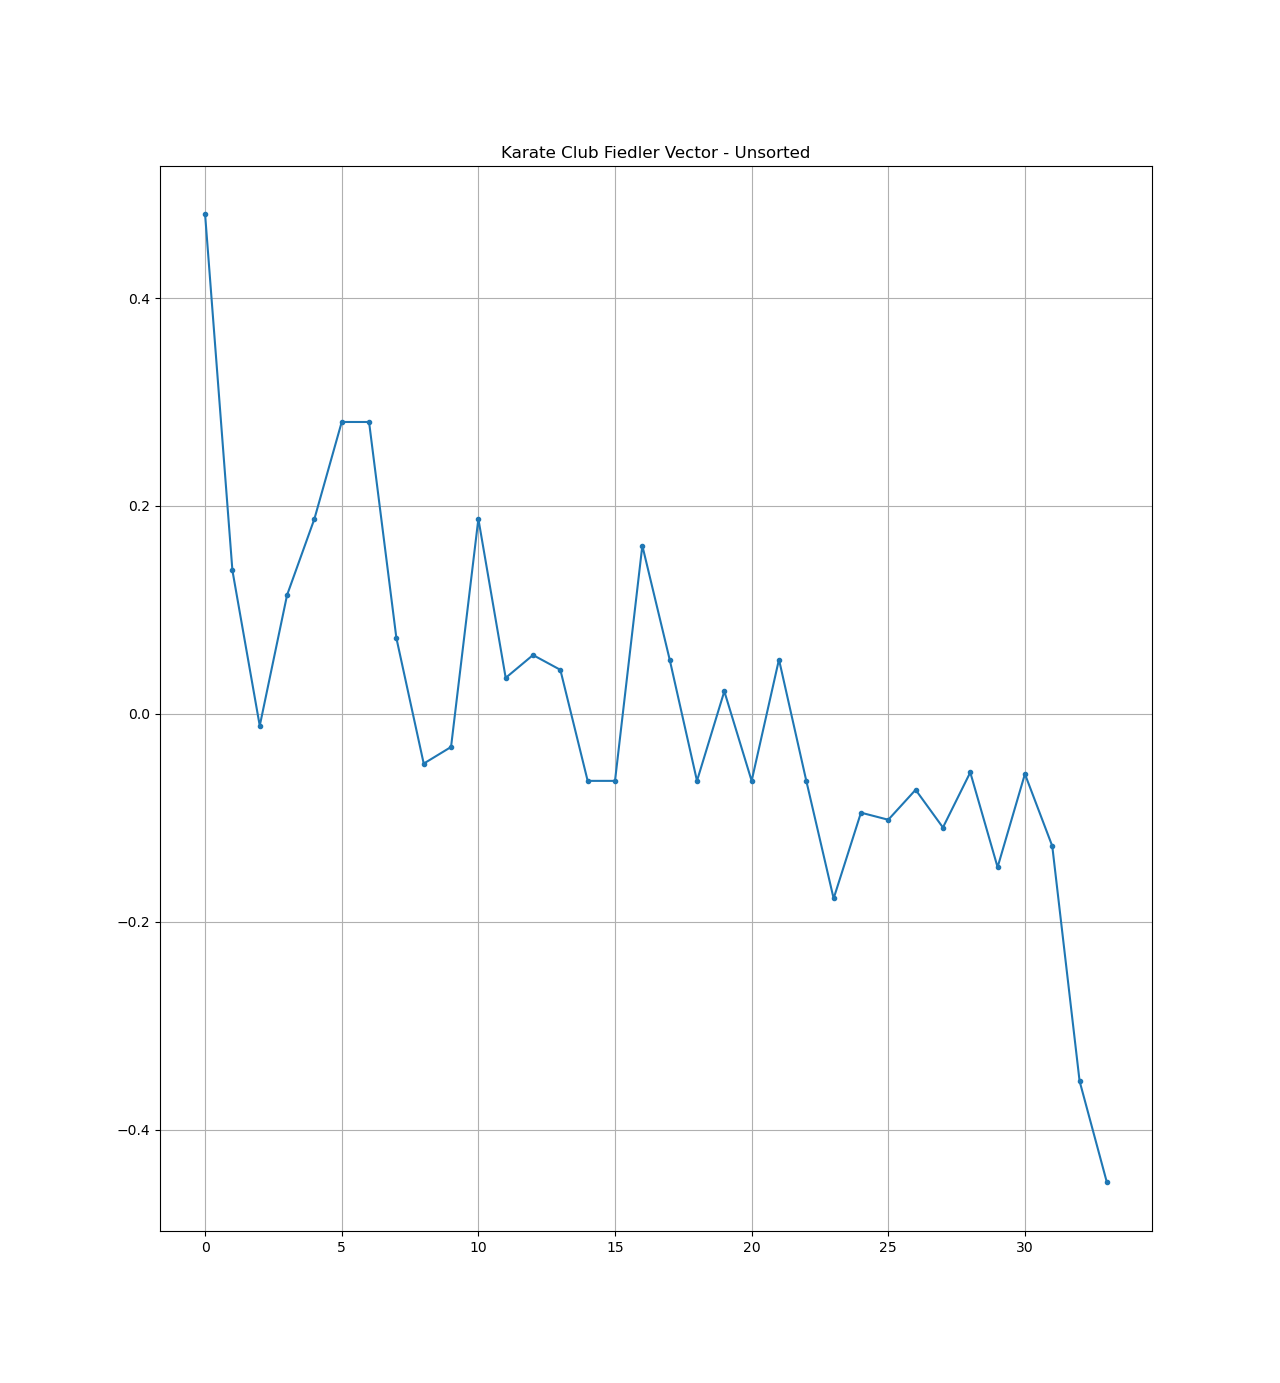
\includegraphics[width=\textwidth]{figures/karate_fiedler_unsorted.png}
\caption{Plot of the Fiedler Vector of the Karate Club. The split between
negative and positive values is much less dramatic but nonetheless still visible.}
\label{fig:karatefiedlerplot}
\end{subfigure}
%add desired spacing between images, e. g. ~, \quad, \qquad, \hfill etc. 
%(or a blank line to force the subfigure onto a new line)
%\caption{}
%\label{fig:exampleCoolWarmClustering}
\end{framed}
\end{figure}



%tests
%\section{Tests}
%Here is a lemma with a reference
%\begin{lemma}
%\label{lemma:foo}
%This is Lemma Foo
%\begin{proof}
%This is the proof of lemma \ref{lemma:foo}
%\end{proof}
%\end{lemma}
%
%That was a proof of lemma \ref{lemma:foo} is in the appendix.

% references
\section{Reference}
\nocite{slides_from_lecture}
\nocite{cowen2017network}
\nocite{vandin2012discovery}
\nocite{vandin2012discovery}
\nocite{leiserson2015pan}

\printbibliography

\listoffigures
\listoftables


\end{document}

